\subsection{Phân tích tập dữ liệu chỉ bao gồm các quan sát có cột "emailtotal" không phải giá trị null}

\begin{figure}[H]
    \centering
    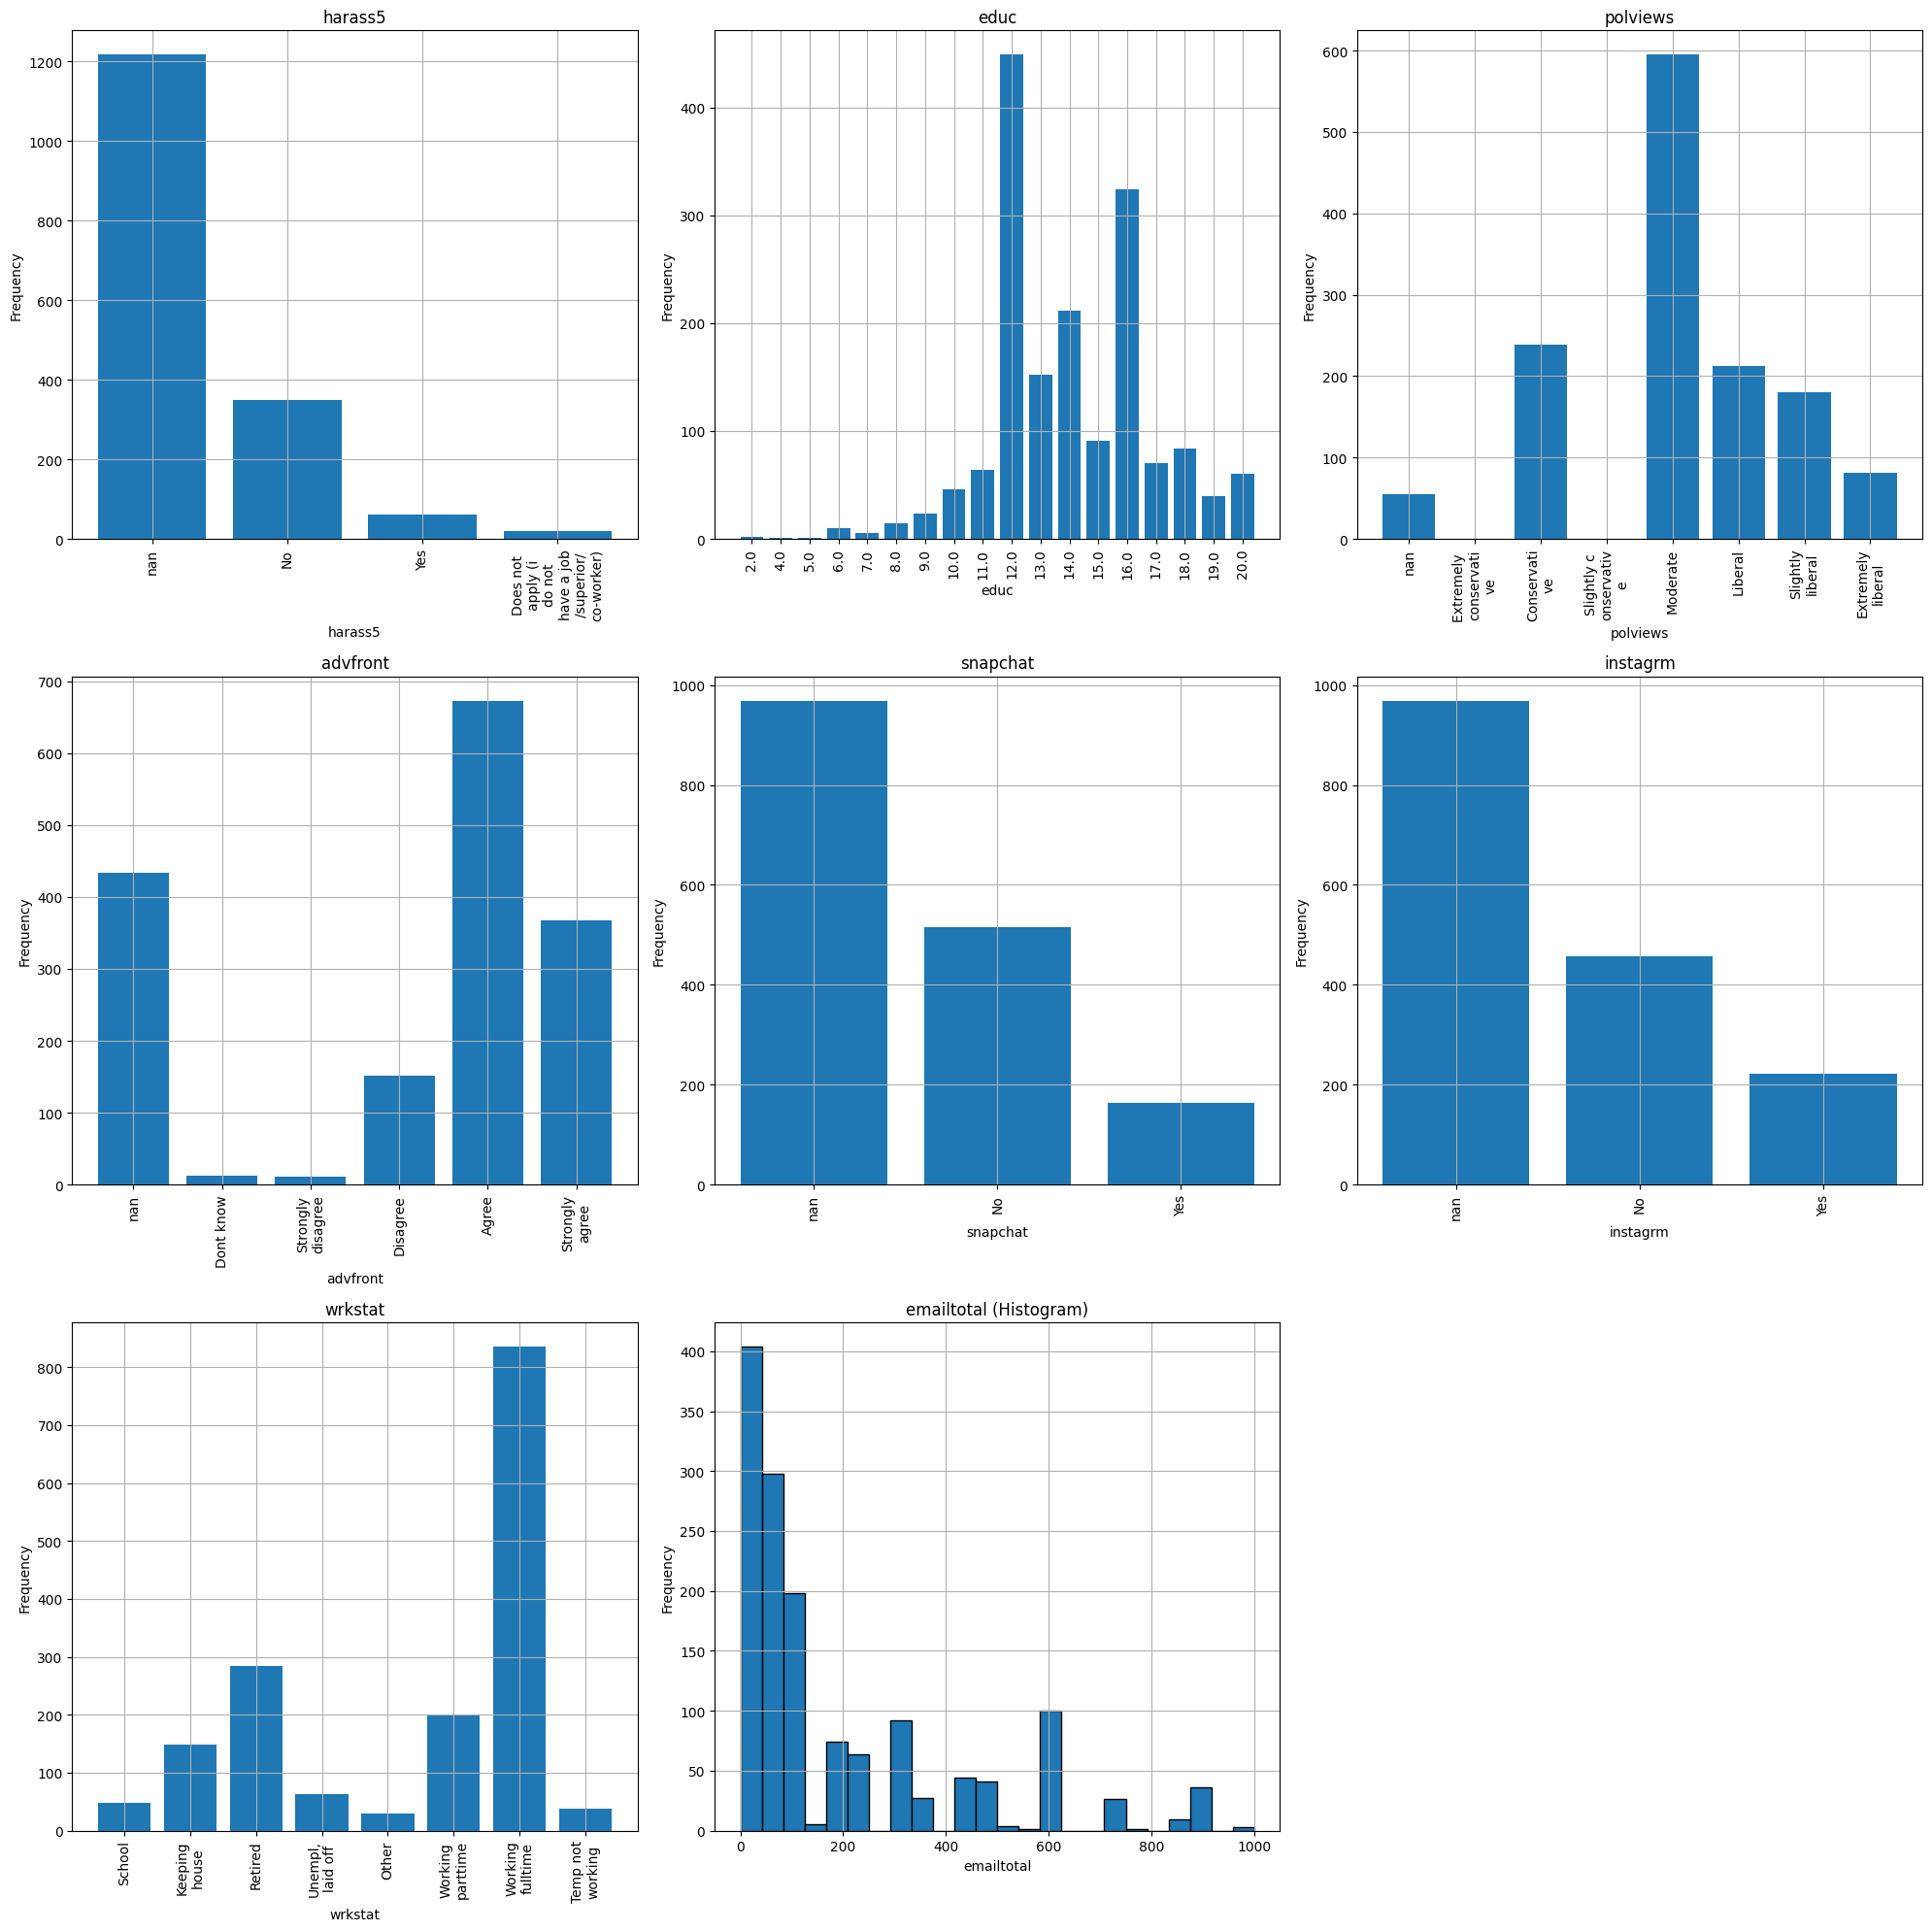
\includegraphics[width=0.6\textwidth]{figures/Thanh/Data_Analysis/Non_null_frequency_of_unique_values_of_columns.png}
    \caption{Tần suất của từng giá trị của từng cột trong tập dữ liệu chỉ bao gồm các quan sát có cột "emailtotal" không phải giá trị null}
    \label{fig:Non_null_frequency_of_unique_values_of_columns}
\end{figure}

Hình \ref{fig:Non_null_frequency_of_unique_values_of_columns} cho biết tần suất của từng giá trị của từng cột trong tập dữ liệu chỉ bao gồm các quan sát có cột "emailtotal" không phải giá trị null.
Cột "harass5" có một lượng rất lớn các quan sát có giá trị là null.
Cột "educ" đa số các quan sát có học vấn từ 12 đến 16 năm.
Quan điểm chính trị đa số mọi người có quan điểm trung lập.
Sử dụng các mạng xã hội, đa số các quan sát là null, tỷ lệ người có sử dụng hoặc không sử dụng snapchat hoặc instagrm tương đối bằng nhau.
Đa số mọi người ở tình trạng làm việc toàn thời gian (working fulltime).
Thời gian hàng tuần dành cho email của mọi người đa số dưới 200 phút, một số nhóm nhỏ dành thời gian cho email từ 600 đến 1000 phút trong một tuần.

\begin{figure}[H]
    \centering
    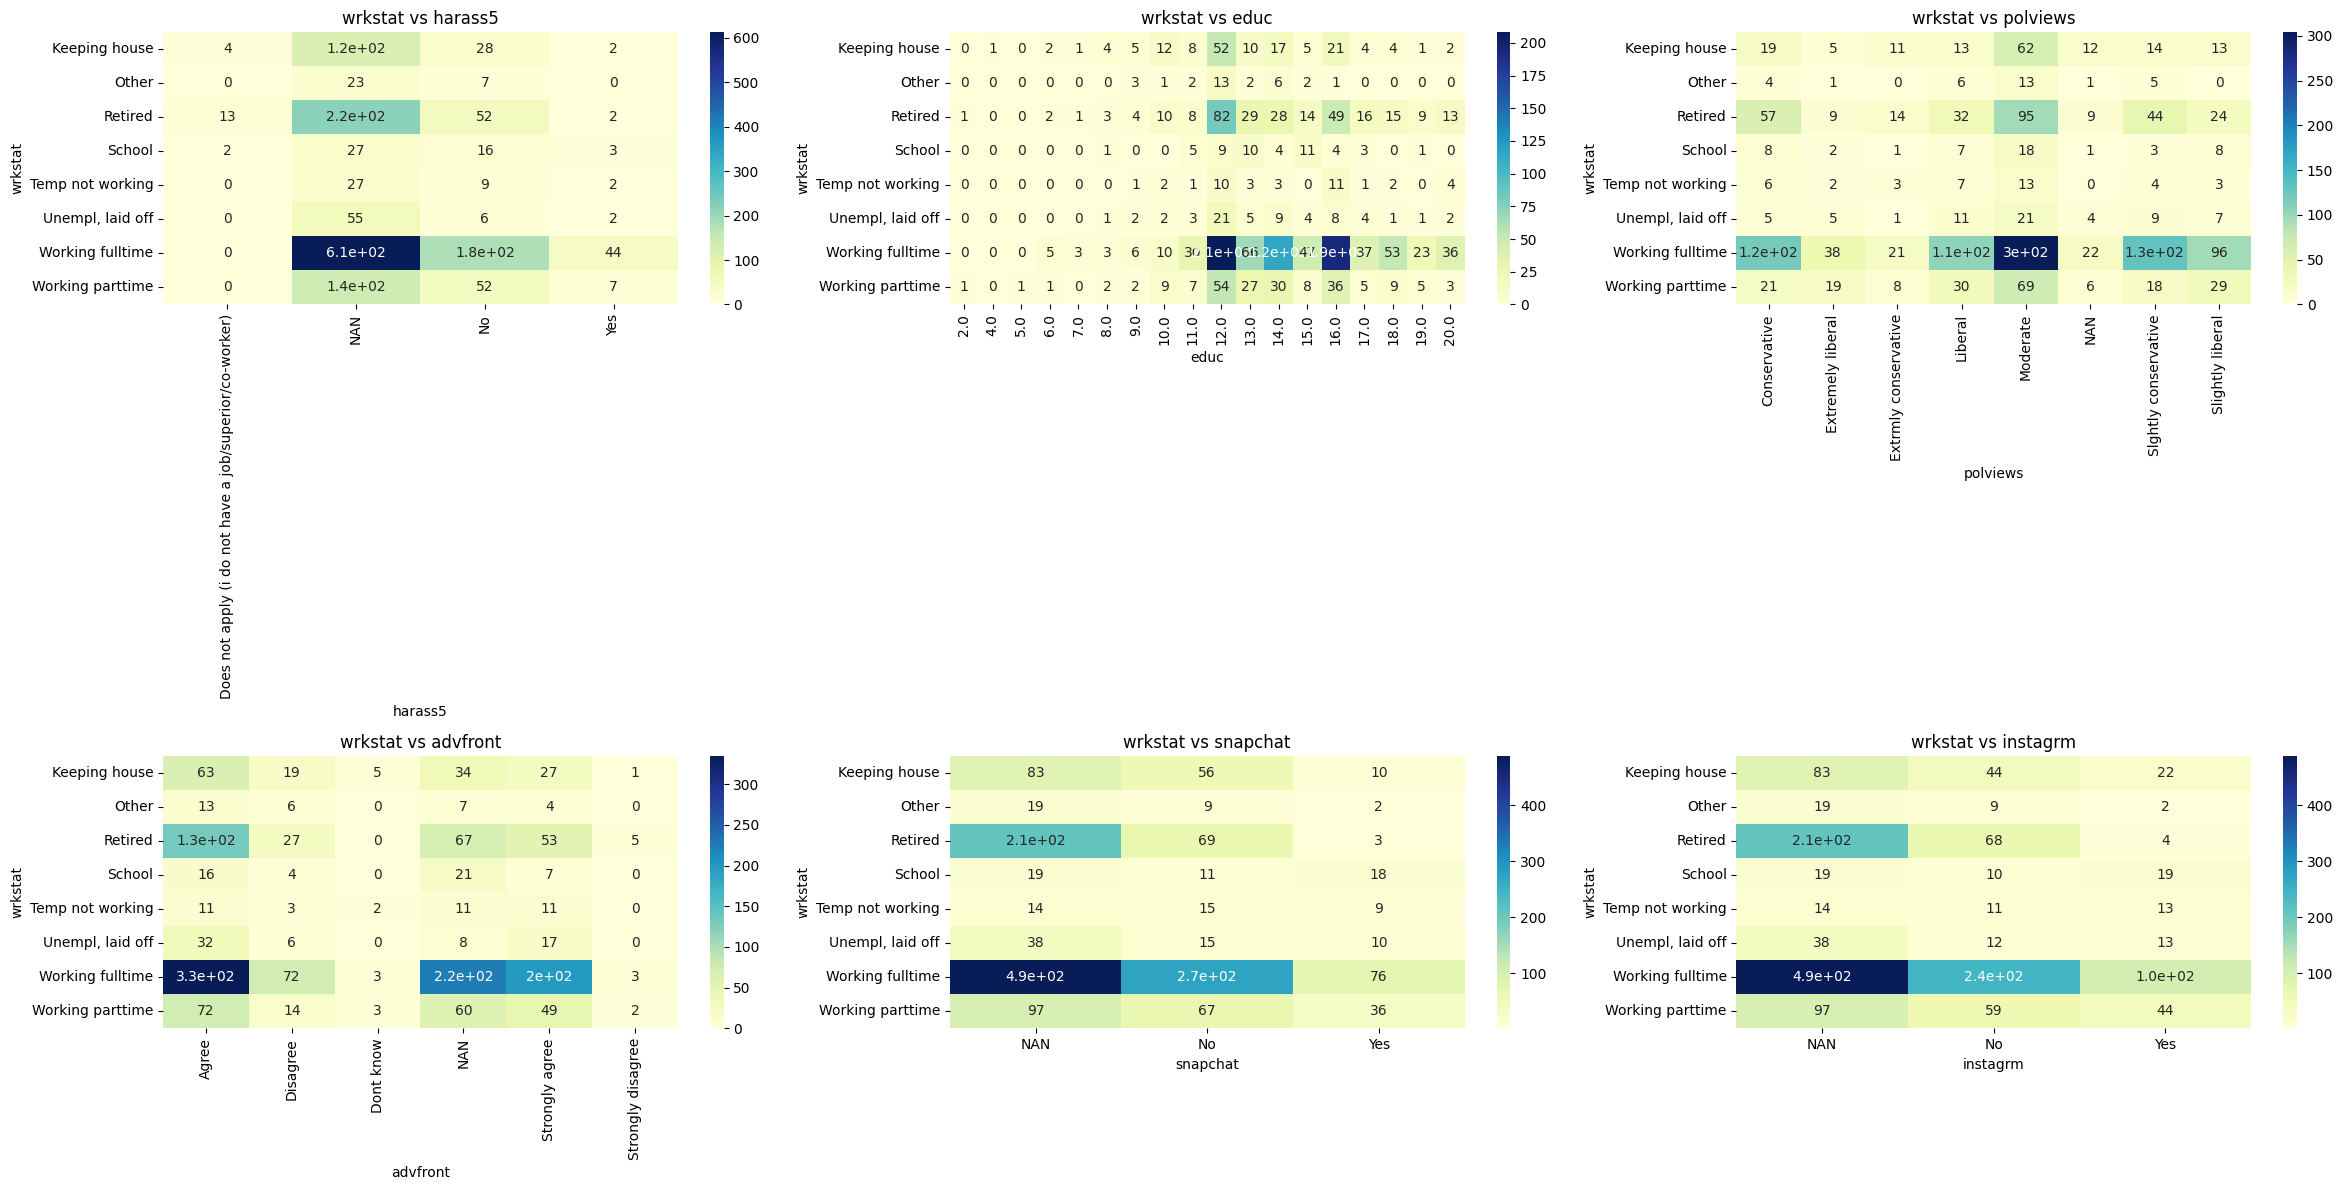
\includegraphics[width=0.8\textwidth]{figures/Thanh/Data_Analysis/Non_null_cooccurrence_matrix_categorical_columns_vs_wrkstat.png}
    \caption{Ma trận đồng xuất hiện của các cột dạng phân loại với cột "wrkstat"}
    \label{fig:Non_null_cooccurrence_matrix_categorical_columns_vs_wrkstat}
\end{figure}

Hình \ref{fig:Non_null_cooccurrence_matrix_categorical_columns_vs_wrkstat} thể hiện các ma trận đồng xuất hiện của các cột dạng phân loại với cột "wrkstat".
Ta nhận thấy đối với từng ma trận đồng xuất hiện, các ô tương ứng với vị trí trạng thái làm việc là toàn thời gian lớn hơn các ô ứng với trạng thái làm việc khác.
Còn tại các cột dạng phân loại, độ lớn các ô theo từng giá trị tương ứng với các cột khá giống với biểu đồ cột ở hình \ref{fig:Non_null_frequency_of_unique_values_of_columns}.

\begin{figure}[H]
    \centering
    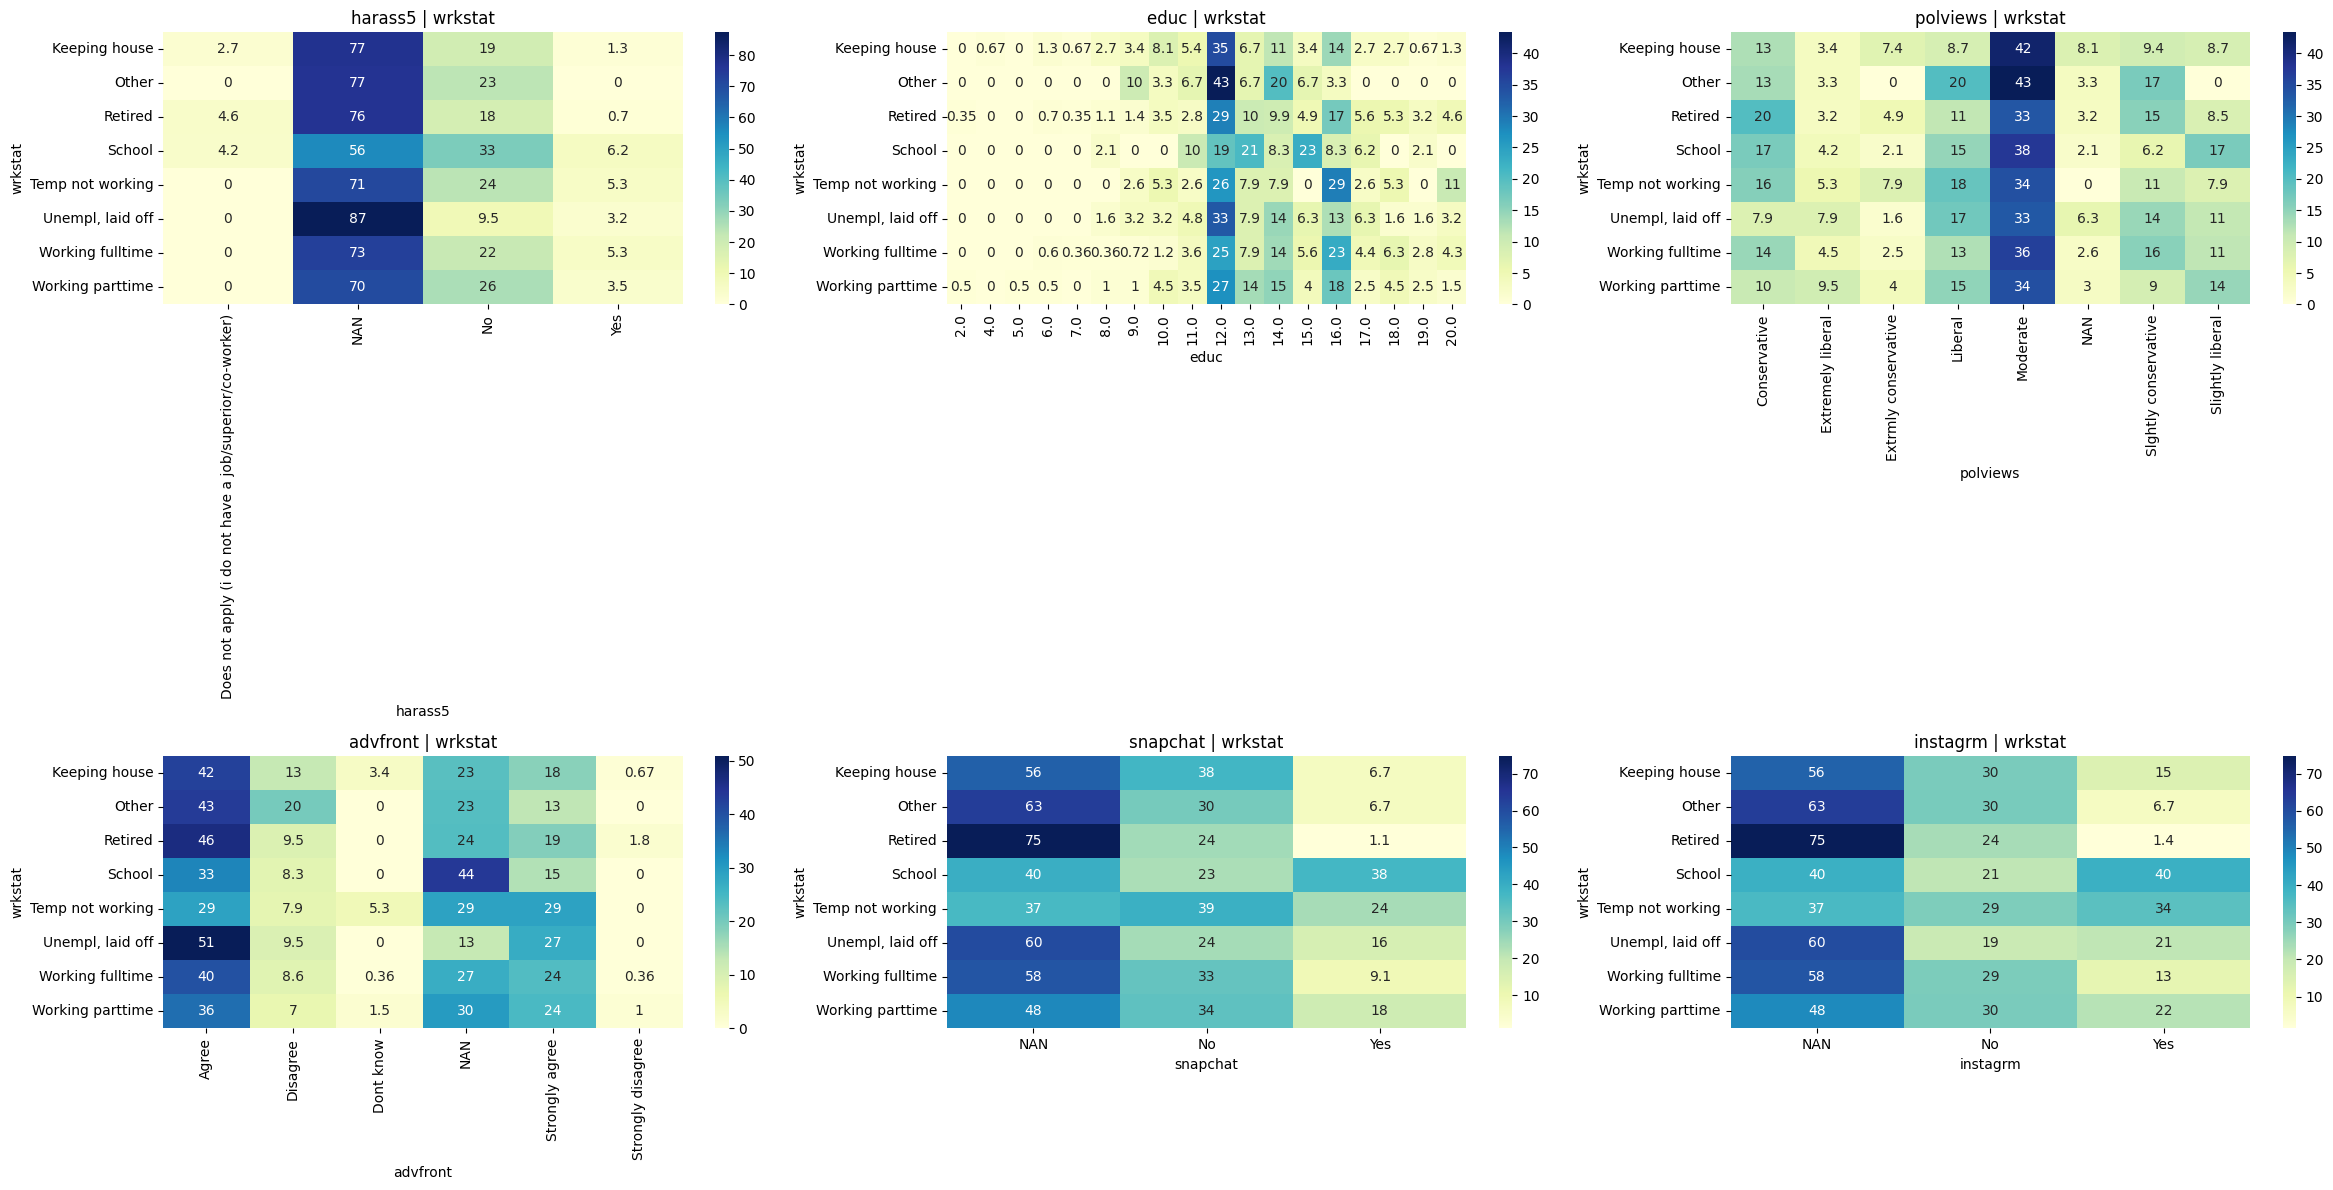
\includegraphics[width=0.6\textwidth]{figures/Thanh/Data_Analysis/Non_null_percentage_matrix_categorical_columns_condition_on_wrkstat.png}
    \caption{Tính bảng tỷ lệ của các giá trị của các cột phân loại khi cố định từng giá trị của trường wrkstat}
    \label{fig:Non_null_percentage_matrix_categorical_columns_condition_on_wrkstat}
\end{figure}

Hình \ref{fig:Non_null_percentage_matrix_categorical_columns_condition_on_wrkstat} cho biết tỷ lệ có điều kiện của các cột dạng phân loại lấy điều kiện trên cột wrkstat.
Ta nhận thấy độ lớn các ô theo từng giá trị tương ứng với các cột khá giống với biểu đồ cột ở hình \ref{fig:Non_null_frequency_of_unique_values_of_columns}.

\begin{figure}[H]
    \centering
    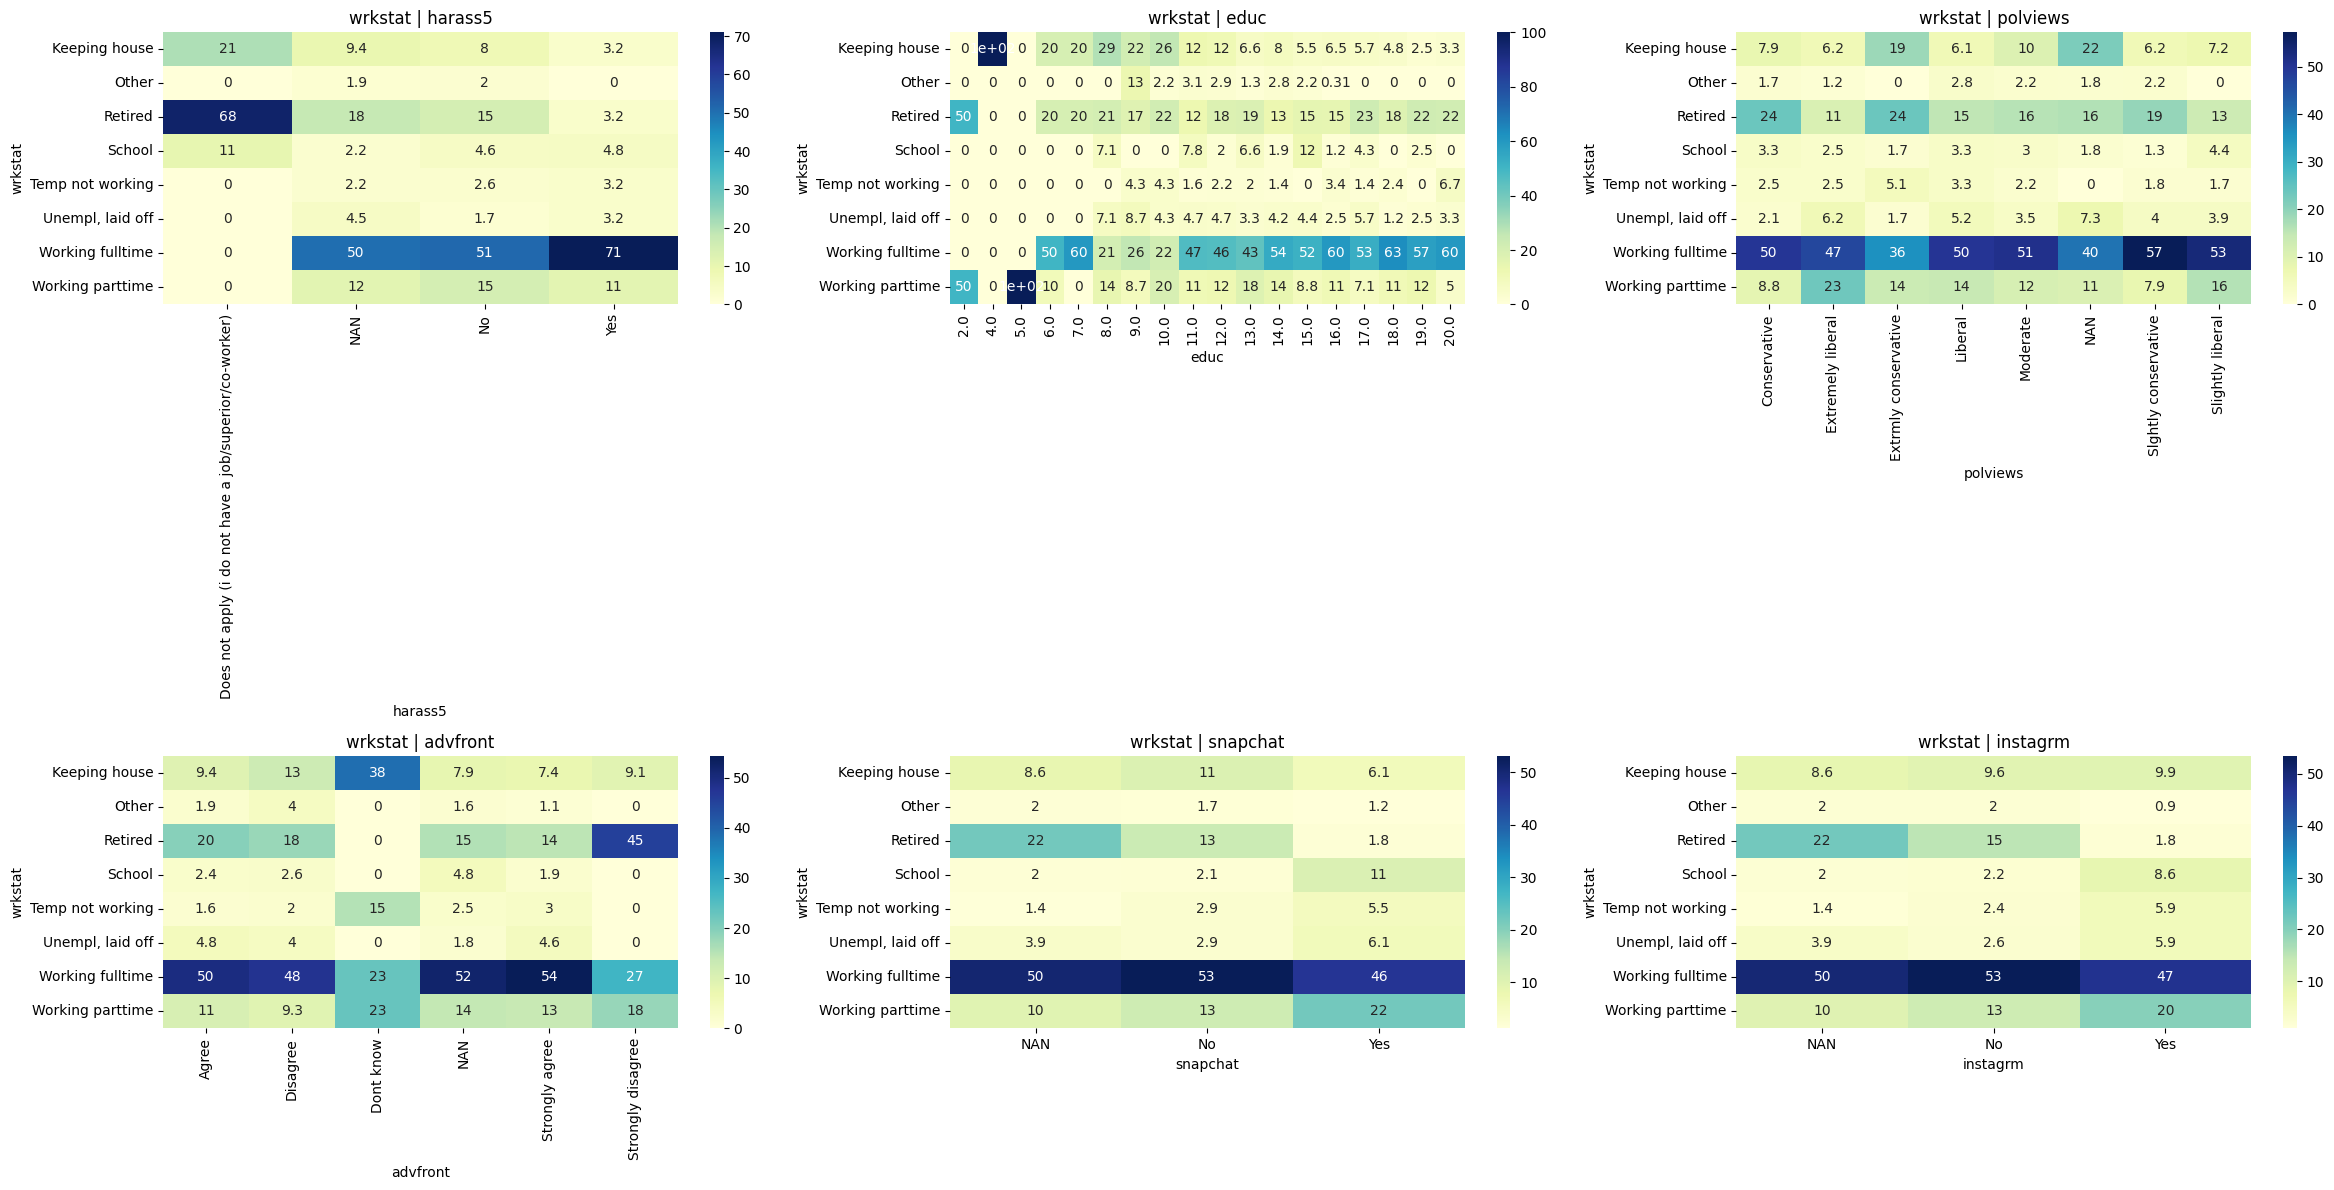
\includegraphics[width=0.6\textwidth]{figures/Thanh/Data_Analysis/Non_null_percentage_matrix_categorical_wrkstat_condition_on_columns.png}
    \caption{Tỷ lệ của các giá trị của cột wrkstat khi cố định từng giá trị của các cột dạng phân loại}
    \label{fig:Non_null_percentage_matrix_categorical_wrkstat_condition_on_columns}
\end{figure}

Hình \ref{fig:Non_null_percentage_matrix_categorical_wrkstat_condition_on_columns} biểu diễn Tỷ lệ của các giá trị của cột wrkstat khi cố định từng giá trị của các cột dạng phân loại.
Ta nhận thấy ứng với mỗi giá trị của các cột khác về cơ bản tỷ lệ người đang trong trạng thái làm việc toàn thời gian có tỷ lệ cao nhất trừ một số trường hợp đặc biệt như người không tham gia lao động thì tỷ lệ người đã nghỉ hưu là cao nhất.
Hay những người có thời gian đi học thấp khoảng 2 3 năm thì đa số trong trạng thái làm việc bán thời gian.

\begin{figure}[H]
    \centering
    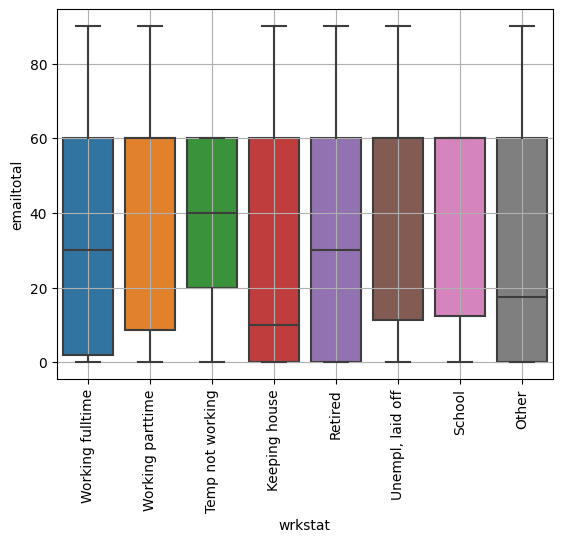
\includegraphics[width=0.5\textwidth]{figures/Thanh/Data_Analysis/Non_null_boxplot_emailtotal_vs_wrkstat_labels.png}
    \caption{Boxplot của thời gian dùng email đối với từng giá trị của cột wrkstat}
    \label{fig:Non_null_boxplot_emailtotal_vs_wrkstat_labels}
\end{figure}

Hình \ref{fig:Non_null_boxplot_emailtotal_vs_wrkstat_labels} thể hiện Boxplot của thời gian dùng email đối với từng giá trị của cột wrkstat.
Không có nhiều sự khác biệt về phân phối của thời gian dùng email đối với từng nhóm trạng thái làm việc.
Phân vị mức 75\% của các nhóm đều rơi vào khoảng 60 phút một tuần.

\begin{table}[ht]
    \centering
    \begin{tabular}{|l|l|}
    \hline
    Cột & p-value \\
    \hline
    harass5 & $4.49 \times 10^{-9}$ \\
    \hline
    educ & $2.19 \times 10^{-7}$ \\
    \hline
    polviews & $0.00242$ \\
    \hline
    advfront & $0.000247$ \\
    \hline
    snapchat & $2.89 \times 10^{-18}$ \\
    \hline
    instagrm & $7.18 \times 10^{-17}$ \\
    \hline
    \end{tabular}
    \caption{Bảng chisquare test kiểm tra tính độc lập của từng cột dạng biến phân loại với cột trạng thái làm việc wrkstat}
    \label{tab:Non_null_chisquare_test}
\end{table}

Ta sử dụng kiểm định chisquare để kiểm tra tính độc lập của từng cột dạng biến phân loại với cột trạng thái làm việc wrkstat.
Các giá trị p-value được thể hiện ở trên bảng \ref{tab:Non_null_chisquare_test}.
Ta nhận thấy tất cả các giá trị p-value tương ứng với từng cặp giữa các cột dạng biến phân loại và cột trạng thái làm việc đều nhỏ hơn 0.05.
Vậy với mức ý nghĩa 0.05, từng cột dạng biến phân loại không độc lập với cột trạng thái làm việc.

\begin{figure}[H]
    \centering
    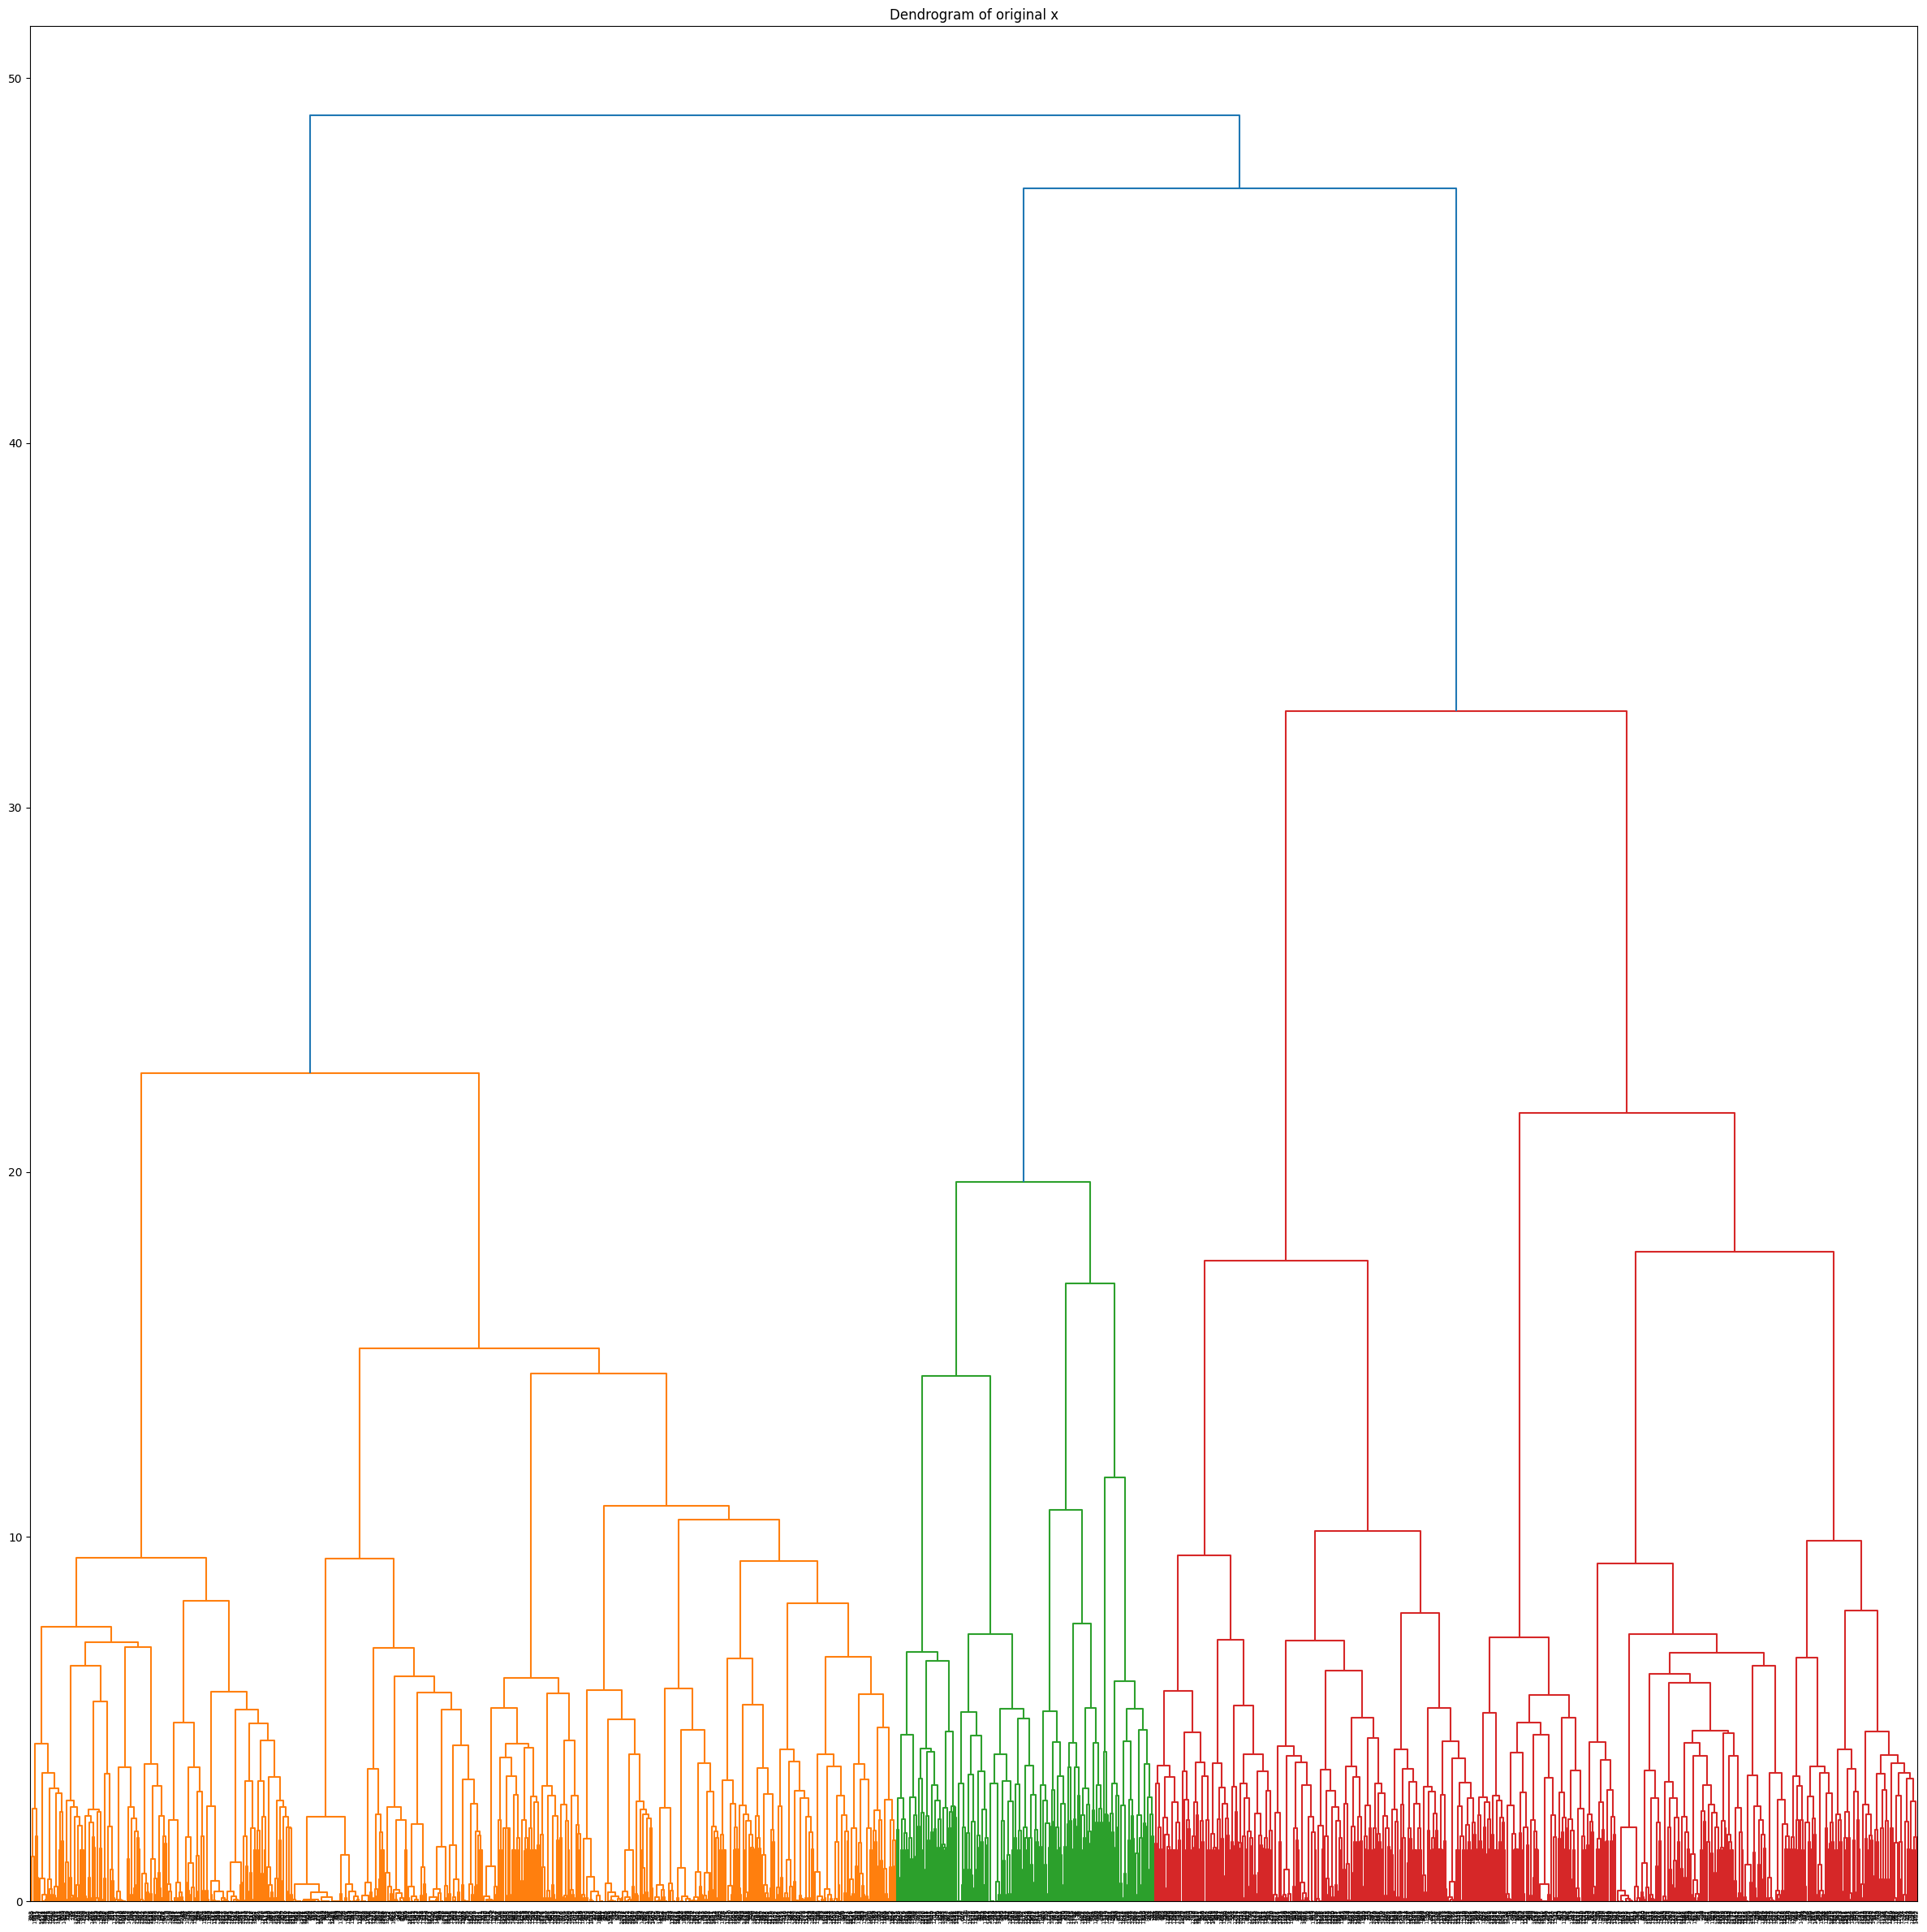
\includegraphics[width=0.6\textwidth]{figures/Thanh/Data_Analysis/Non_null_dendrogram_original_features.png}
    \caption{Dendrogram của tập dữ liệu với biểu diễn là các vector gốc ban đầu}
    \label{fig:Non_null_dendrogram_original_features}
\end{figure}

Để biểu diễn dữ liệu các quan sát thành các vector.
Đối với các cột dạng biến phân loại là harass5, educ, polviews, advfront, snapchat, instagrm ta sử dụng phương pháp one-hot encoding.
Với các giá trị null ta xem như có giá trị là Unknown.
Đối với cột dạng biến lượng là emailtotal ta sử dụng phương pháp chuẩn hóa đưa về trung bình là 0 và phương sai là 1.
Vector cho mỗi quan sát thu được từ phương pháp trên ta gọi là "vector gốc ban đầu".

Hình \ref{fig:Non_null_dendrogram_original_features} thể hiện dendrogram của tập dữ liệu với biểu diễn là các vector gốc ban đầu.
Nhìn sơ bộ, ta nhận thấy có 3 nhóm (cụm) lớn. Hai cụm có số lượng quan sát khá lớn và một cụm có số lượng quan sát nhỏ hơn khá nhiều so với hai cụm còn lại.

\begin{figure}[H]
    \centering
    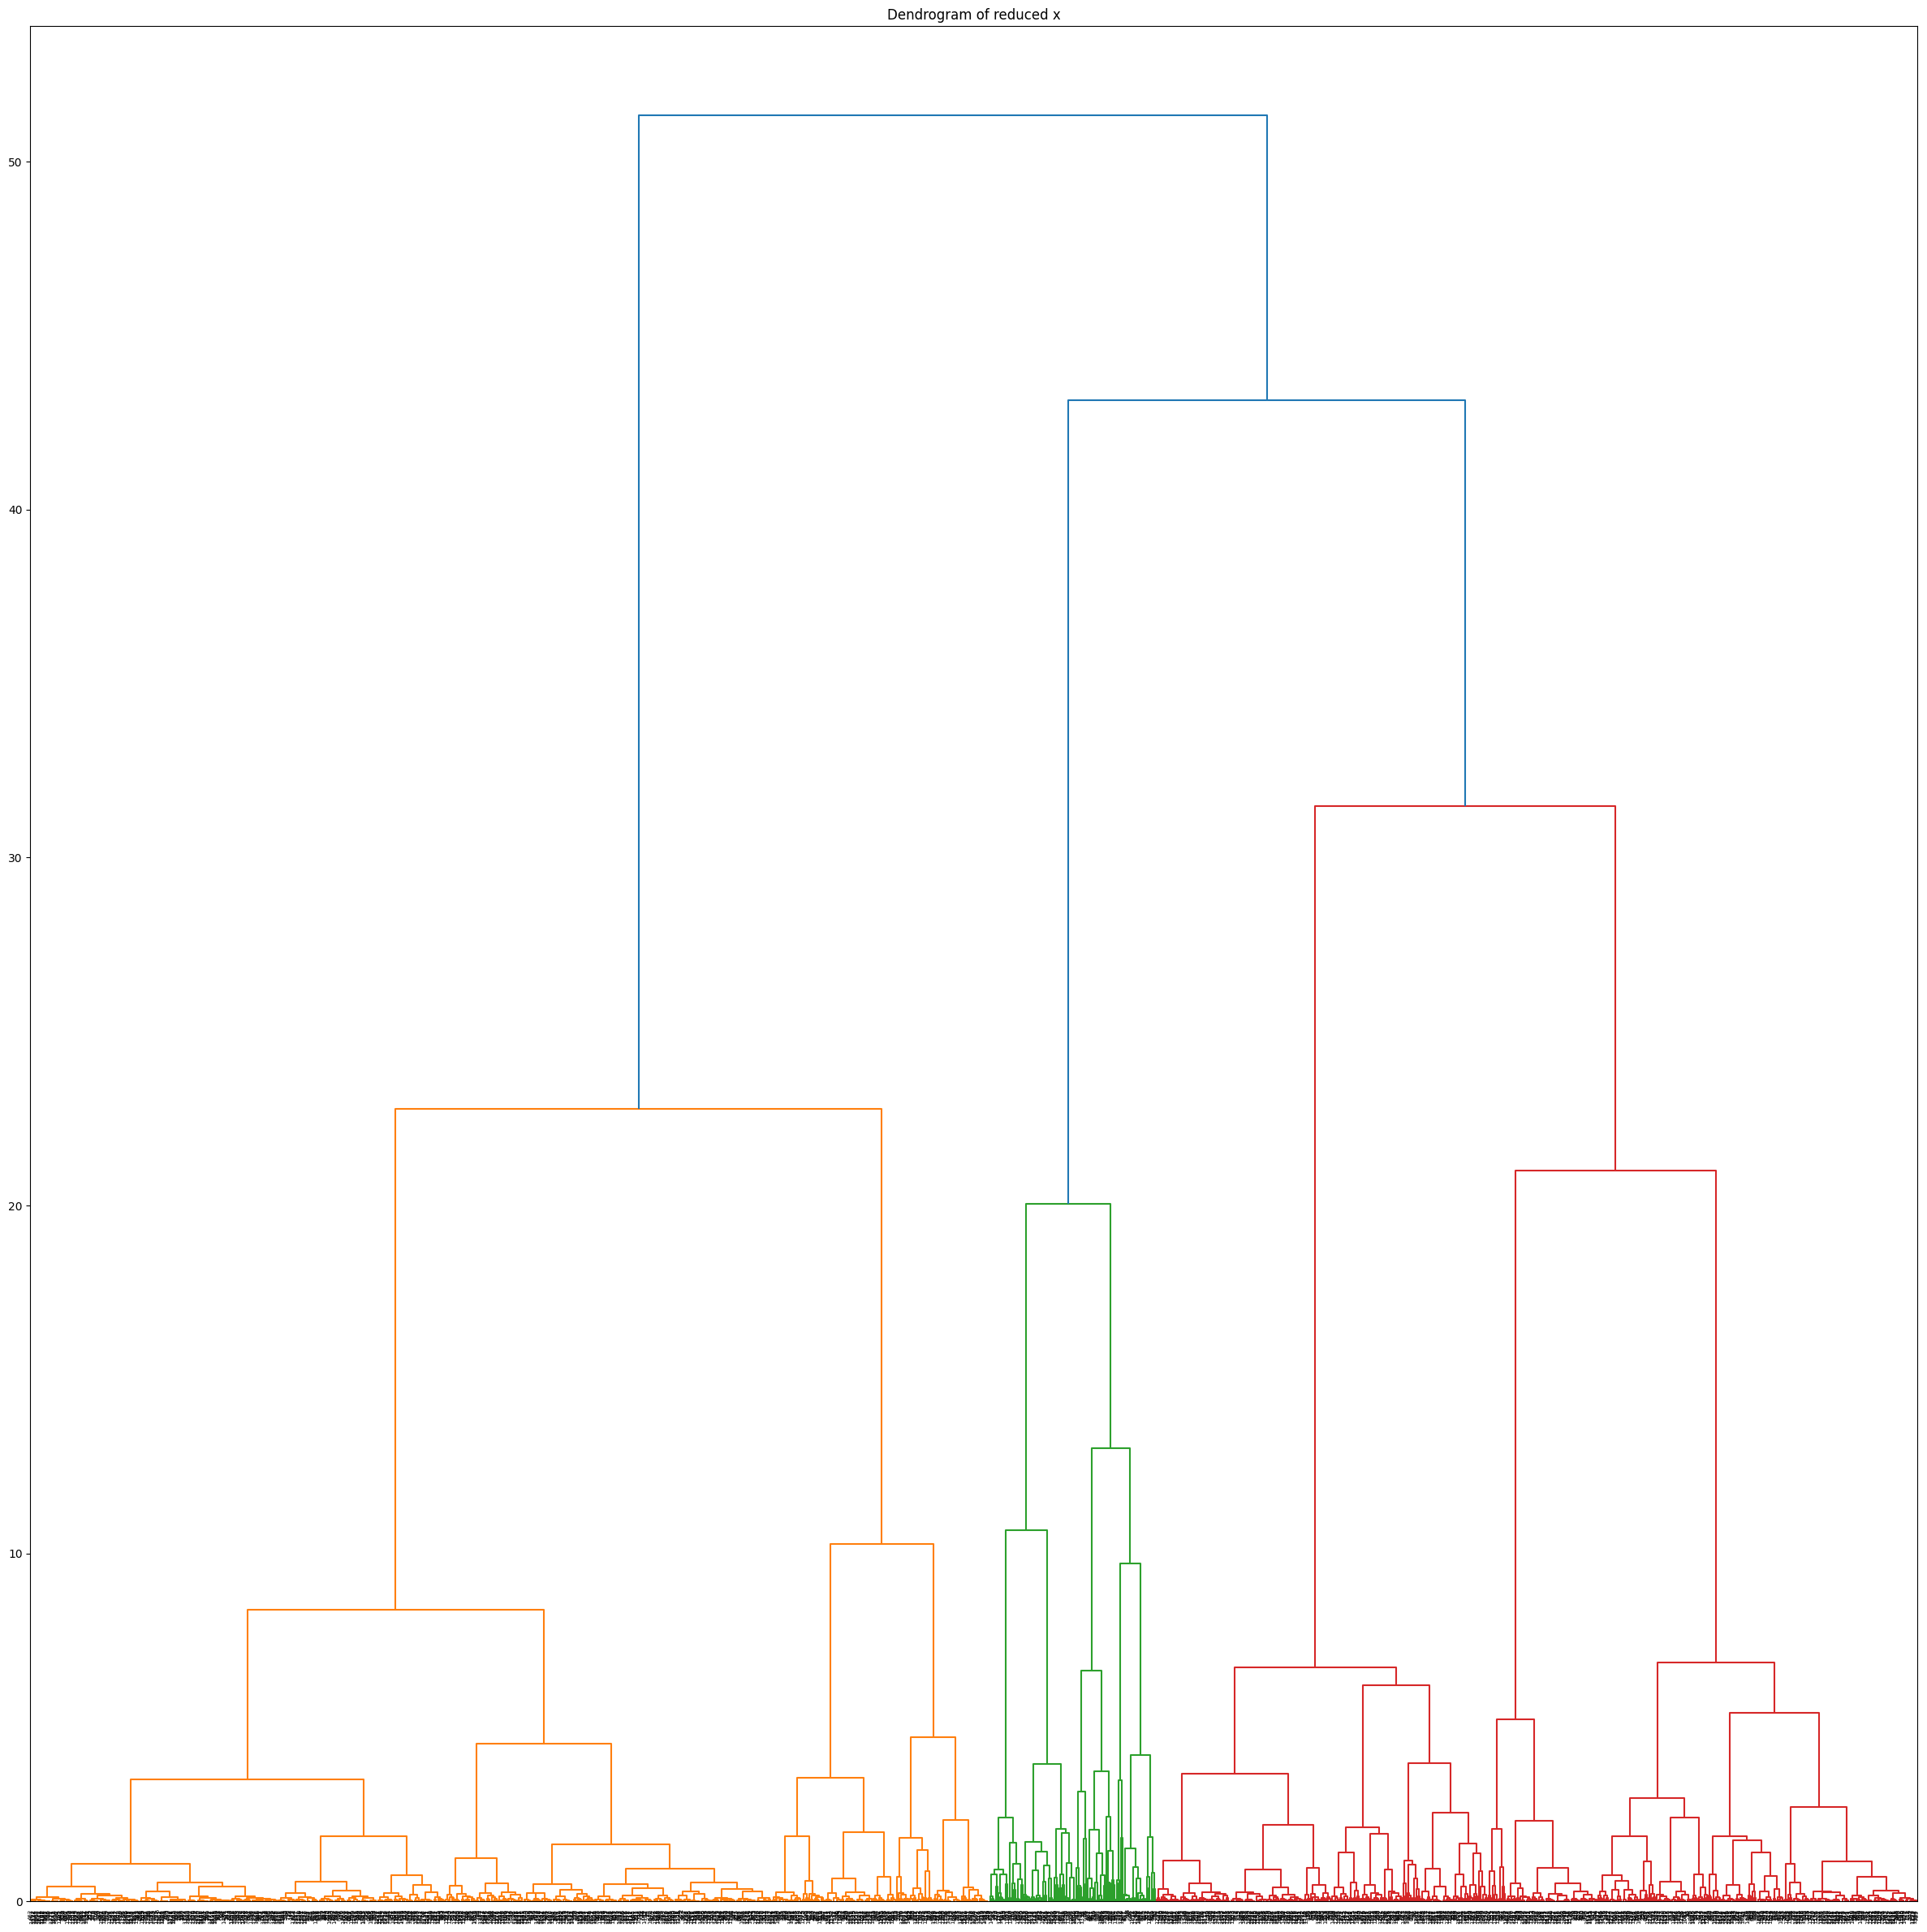
\includegraphics[width=0.6\textwidth]{figures/Thanh/Data_Analysis/Non_null_dendrogram_PCA_features.png}
    \caption{Dendrogram của tập dữ liệu với biểu diễn là các vector thu được từ việc phân tích thành phần chính bằng thuật toán PCA}
    \label{fig:Non_null_dendrogram_PCA_features}
\end{figure}

Ngoài ra ta cũng có thể biểu diễn các quan sát bằng cách phân tích các thành phần chính dùng thuật toán PCA từ các vector gốc ban đầu biểu diễn các quan sát.
Hình \ref{fig:Non_null_dendrogram_PCA_features} biểu diễn dendrogram của tập dữ liệu với biểu diễn của các quan sát là các vector đã được phân tích thành phần chính từ vector gốc ban đầu.
Ta nhận thấy vẫn co 3 nhóm (cụm) lớn. Dendrogram được xây dựng từ tập dữ liệu mà các quan sát được biểu diễn từ phân tích thành phần chính không khác nhiều so với dendrogram được xây dựng từ các vector gốc ban đầu.

Ta sẽ phân tích histogram của các thành phần chính.
Ta phân tích histogram 3 thành phần chính đầu tiên.

\begin{figure}[H]
    \centering
    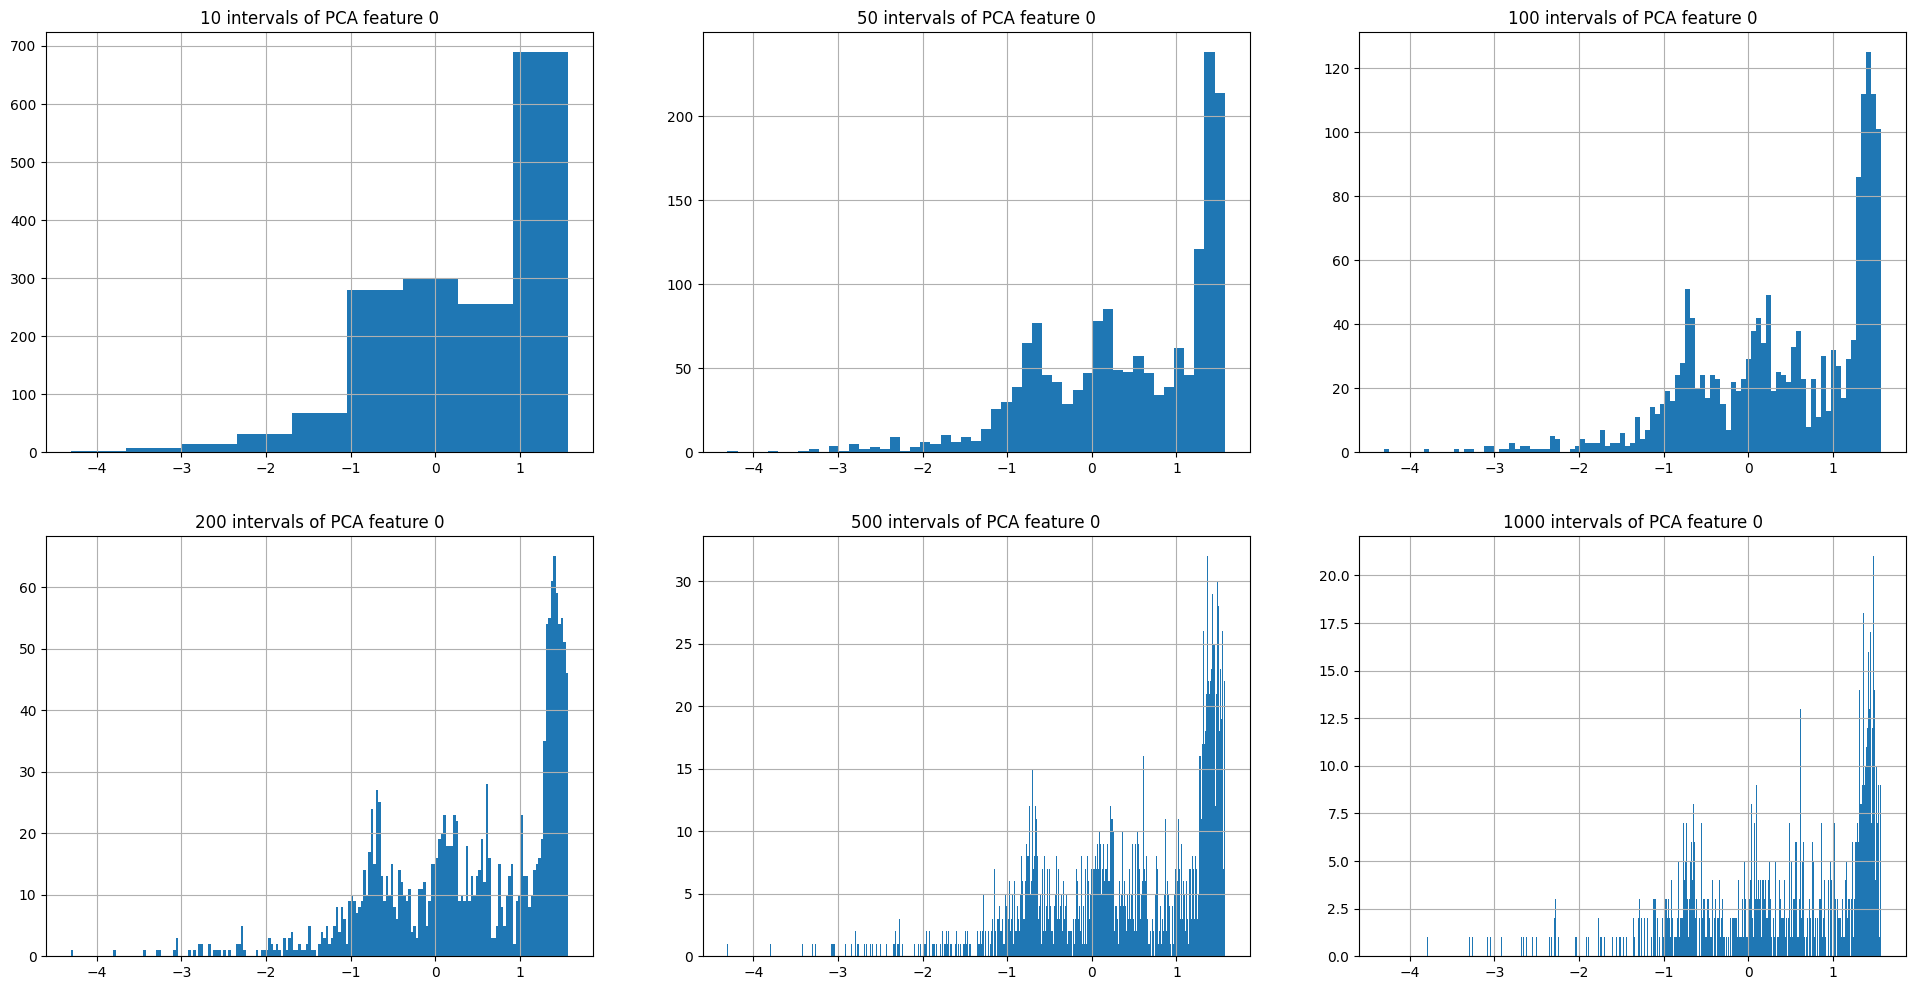
\includegraphics[width=0.75\textwidth]{figures/Thanh/Data_Analysis/Non_null_histogram_PCA_feature_0.png}
    \caption{Histogram của thành phần chính thứ nhất}
    \label{fig:Non_null_histogram_PCA_feature_0}
\end{figure}

Hình \ref{fig:Non_null_histogram_PCA_feature_0} biểu diễn histogram ứng với độ lớn khác nhau của các bins khác nhau.
Ta nhận thấy histogram có 3 đỉnh gợi ý có 3 nhóm các quan sát khi nhìn từ thành phần chính thứ nhất.
Kết quả tương đối tương đồng với dendrogram đã được biểu diễn ở các hình \ref{fig:Non_null_dendrogram_original_features} và \ref{fig:Non_null_dendrogram_PCA_features}.

\begin{figure}[H]
    \centering
    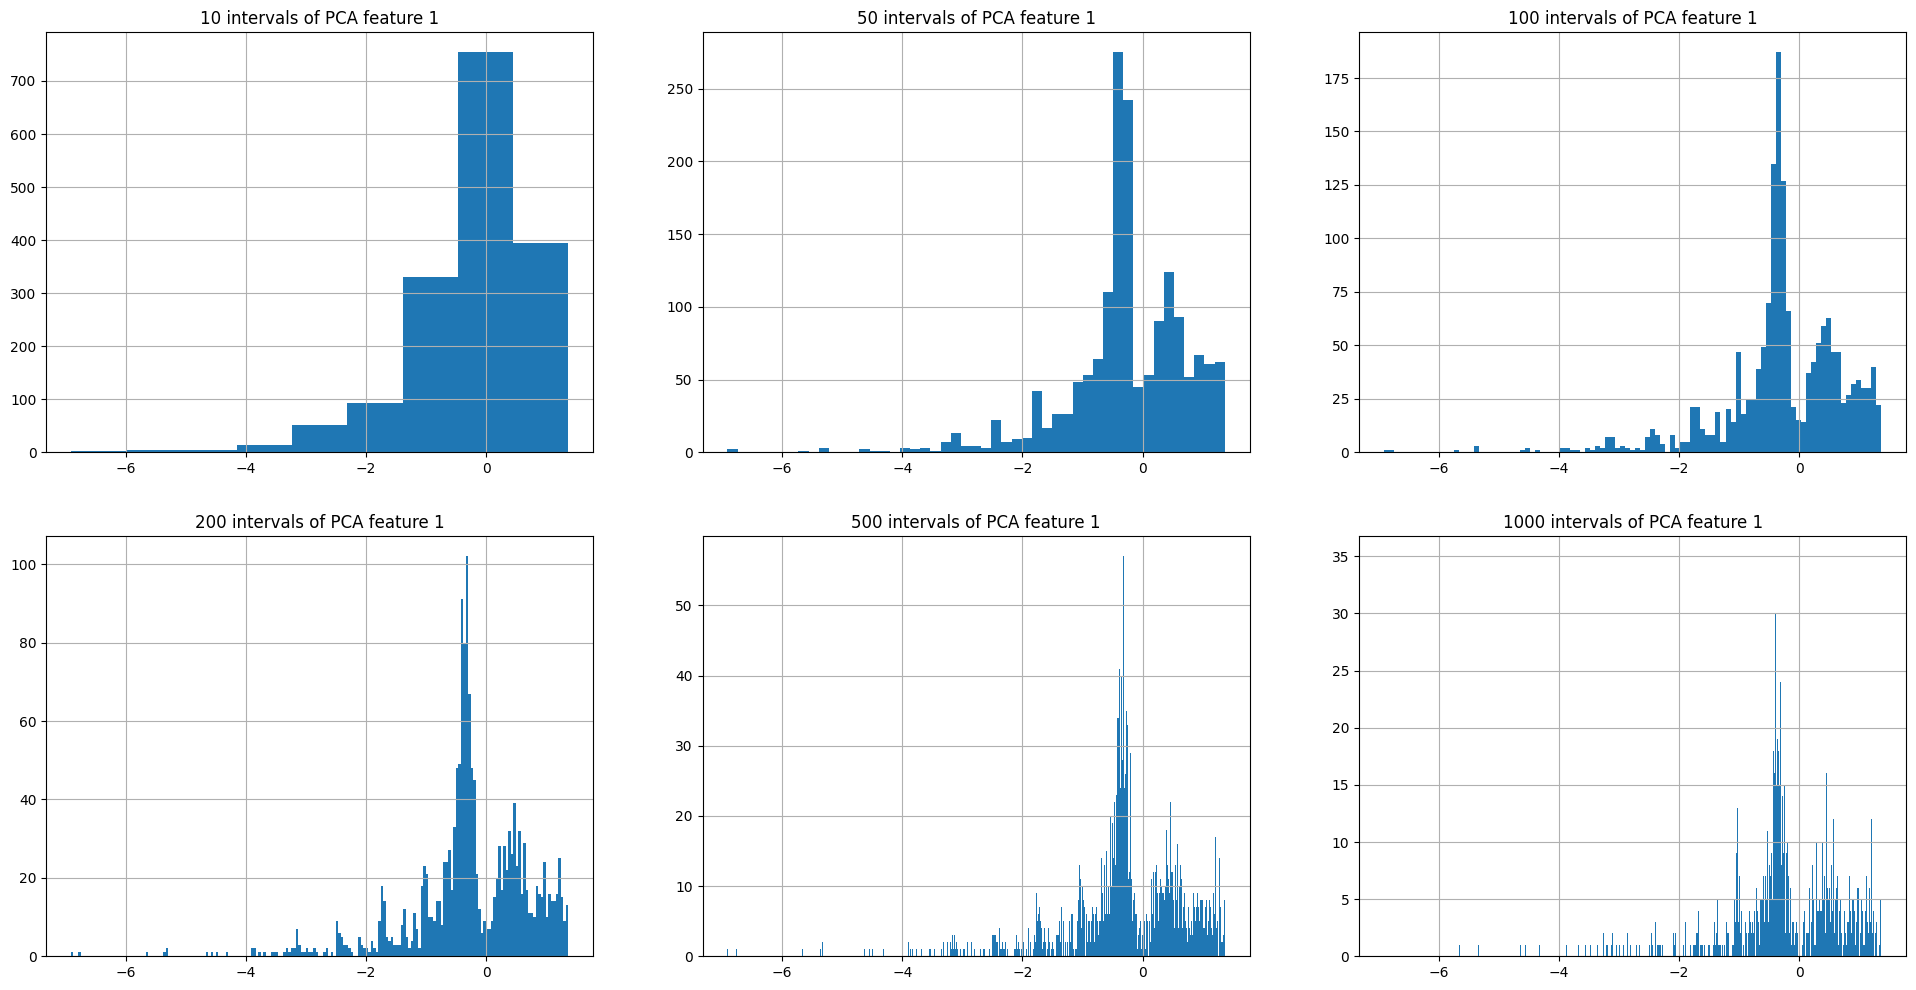
\includegraphics[width=0.75\textwidth]{figures/Thanh/Data_Analysis/Non_null_histogram_PCA_feature_1.png}
    \caption{Histogram của thành phần chính thứ hai}
    \label{fig:Non_null_histogram_PCA_feature_1}
\end{figure}

Hình \ref{fig:Non_null_histogram_PCA_feature_1} biểu diễn histogram ứng với độ lớn khác nhau của các bins khác nhau của thành phần chính thứ hai.
Ta nhận thấy histogram có 3 nhóm lớn nếu nhìn từ thành phần chính thứ hai

\begin{figure}[H]
    \centering
    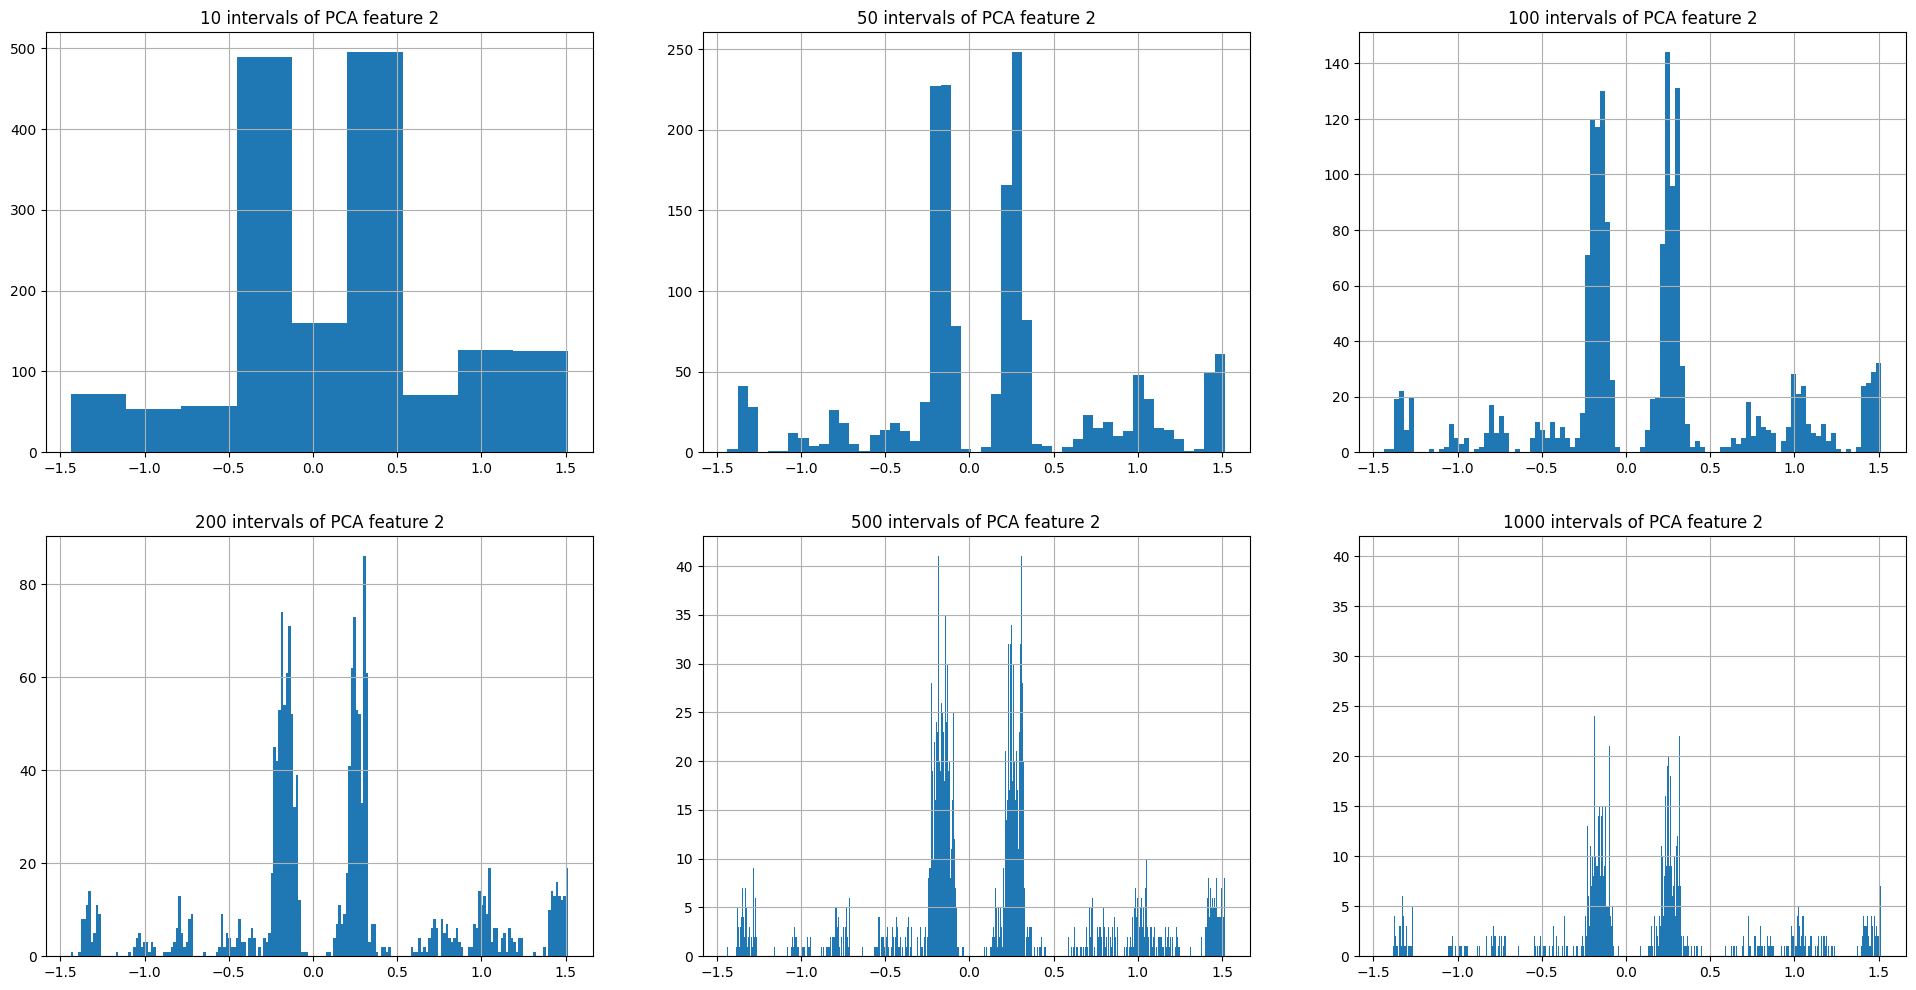
\includegraphics[width=0.75\textwidth]{figures/Thanh/Data_Analysis/Non_null_histogram_PCA_feature_2.png}
    \caption{Histogram của thành phần chính thứ ba}
    \label{fig:Non_null_histogram_PCA_feature_2}
\end{figure}

Hình \ref{fig:Non_null_histogram_PCA_feature_2} biểu diễn histogram ứng với độ lớn khác nhau của các bins khác nhau của thành phần chính thứ ba.
Ta thấy có hai đỉnh chính lớn và một vài đỉnh phụ nhỏ xung quanh nếu nhìn từ thành phần chính thứ backend

Ta sẽ thử vẽ các histogram của các thành phần chính tương ứng với từng giá trị dữ liệu trong cột trạng thái làm việc wrkstat.

\begin{figure}[H]
    \centering
    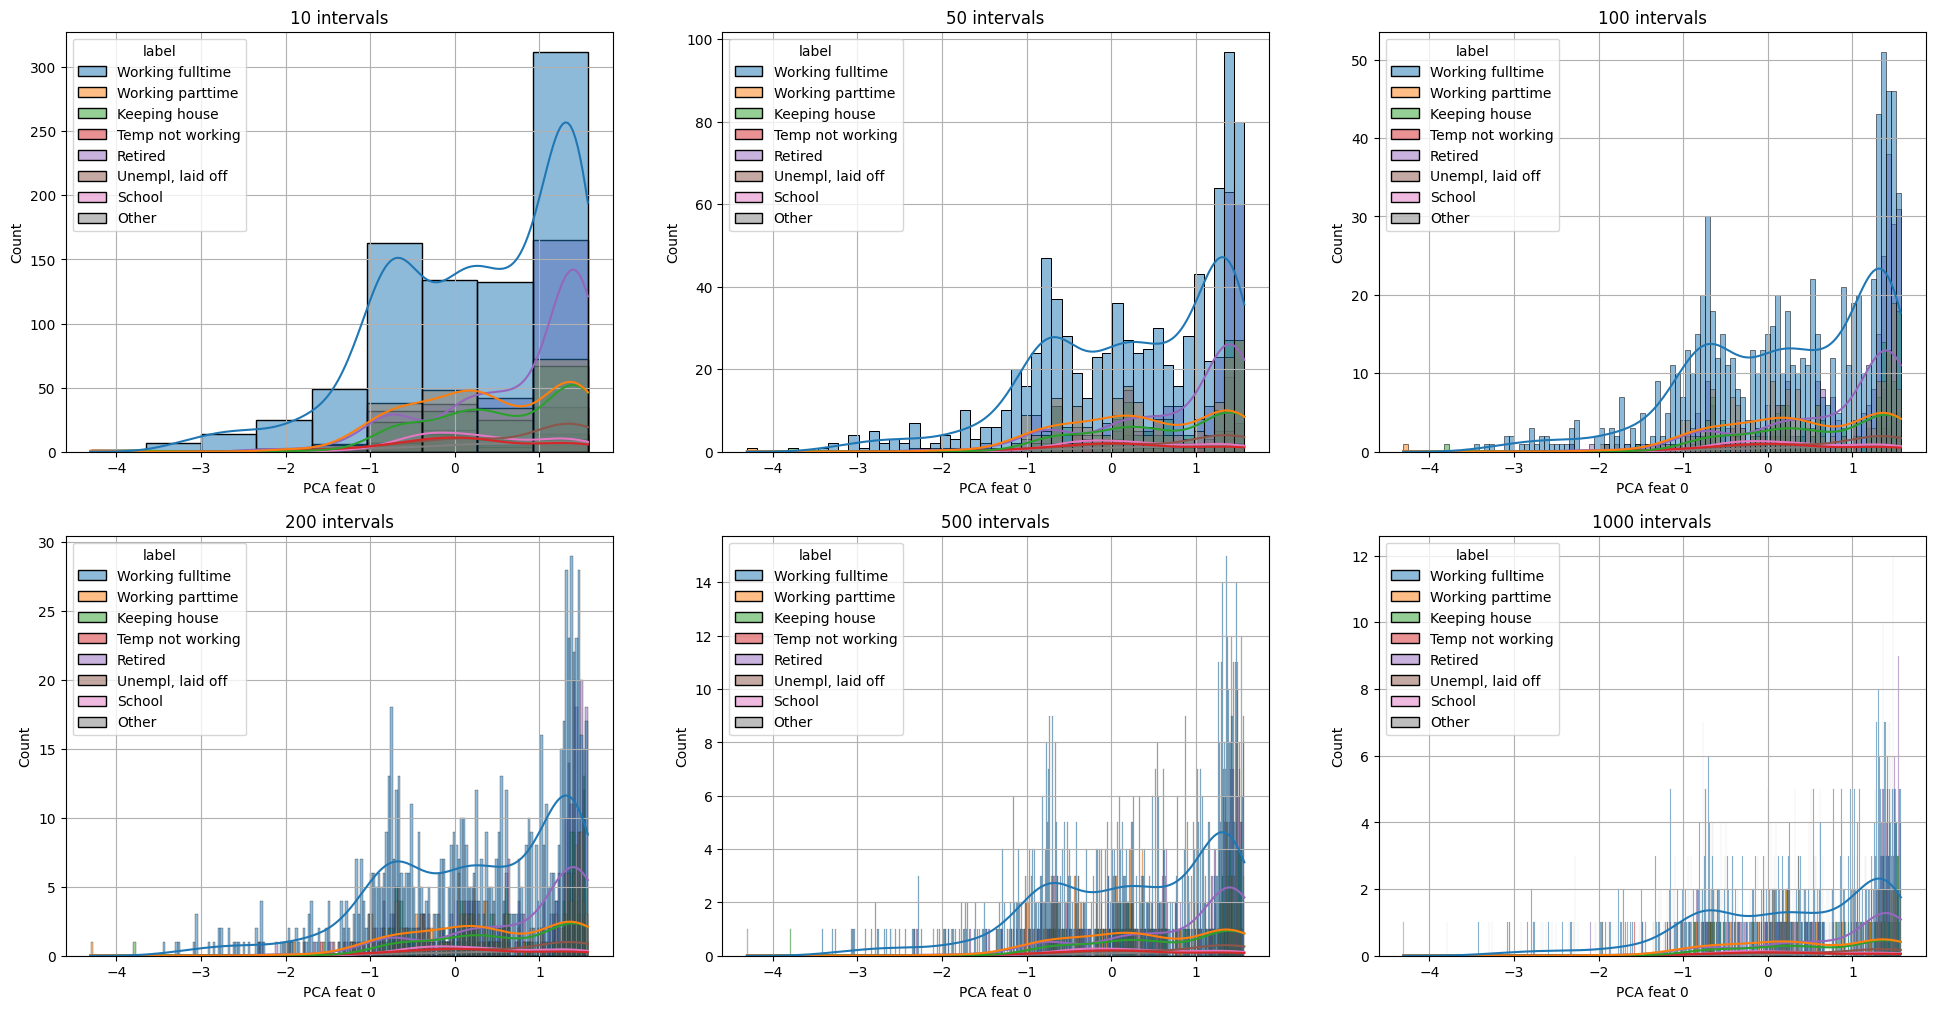
\includegraphics[width=0.75\textwidth]{figures/Thanh/Data_Analysis/Non_null_histogram_PCA_feature_0_vs_wrkstat_labels.png}
    \caption{Histogram của thành phần chính thứ nhất tương ứng với từng giá trị dữ liệu trong cột trạng thái làm việc wrkstat}
    \label{fig:Non_null_histogram_PCA_feature_0_vs_wrkstat_labels}
\end{figure}

Hình \ref{fig:Non_null_histogram_PCA_feature_0_vs_wrkstat_labels} biểu diễn histogram của thành phần chính thứ nhất tương ứng với từng giá trị dữ liệu trong cột trạng thái làm việc wrkstat.
Ta nhận thấy một điều phân phối của histogram của thành phần chính thứ nhất theo các nhóm tương ứng với giá trị trong cột wrkstat gần như cùng hình dạng và trộn lẫn hoàn toàn vào nhau.
Các phân phối cùng đạt cực đại hoặc cực tiểu tại các giá trị trên trục hoành gần như trung nhau.
Ta gần như không nhận thấy sự khác biệt nào về phân phối của thành phần chính thứ nhất theo các nhóm giá trị trong cột wrkstat.

\begin{figure}[H]
    \centering
    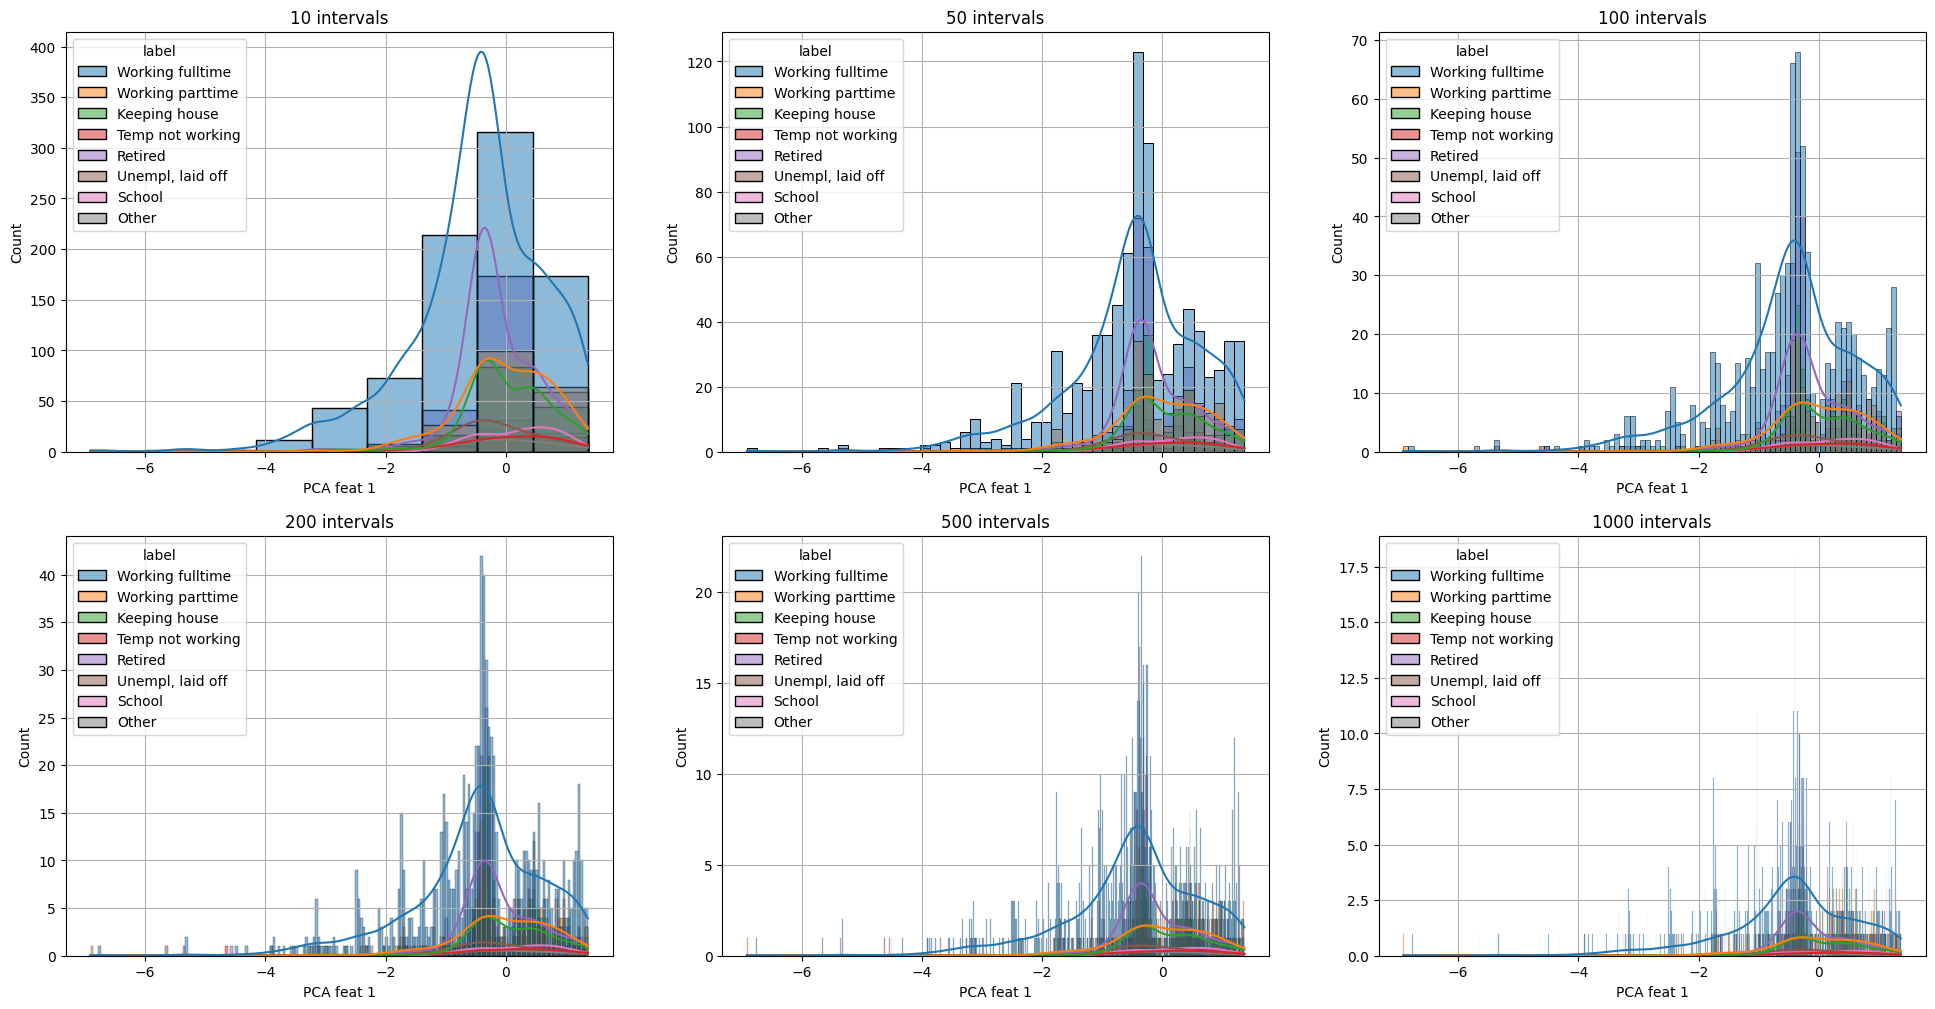
\includegraphics[width=0.75\textwidth]{figures/Thanh/Data_Analysis/Non_null_histogram_PCA_feature_1_vs_wrkstat_labels.png}
    \caption{Histogram của thành phần chính thứ hai tương ứng với từng giá trị dữ liệu trong cột trạng thái làm việc wrkstat}
    \label{fig:Non_null_histogram_PCA_feature_1_vs_wrkstat_labels}
\end{figure}

\begin{figure}[H]
    \centering
    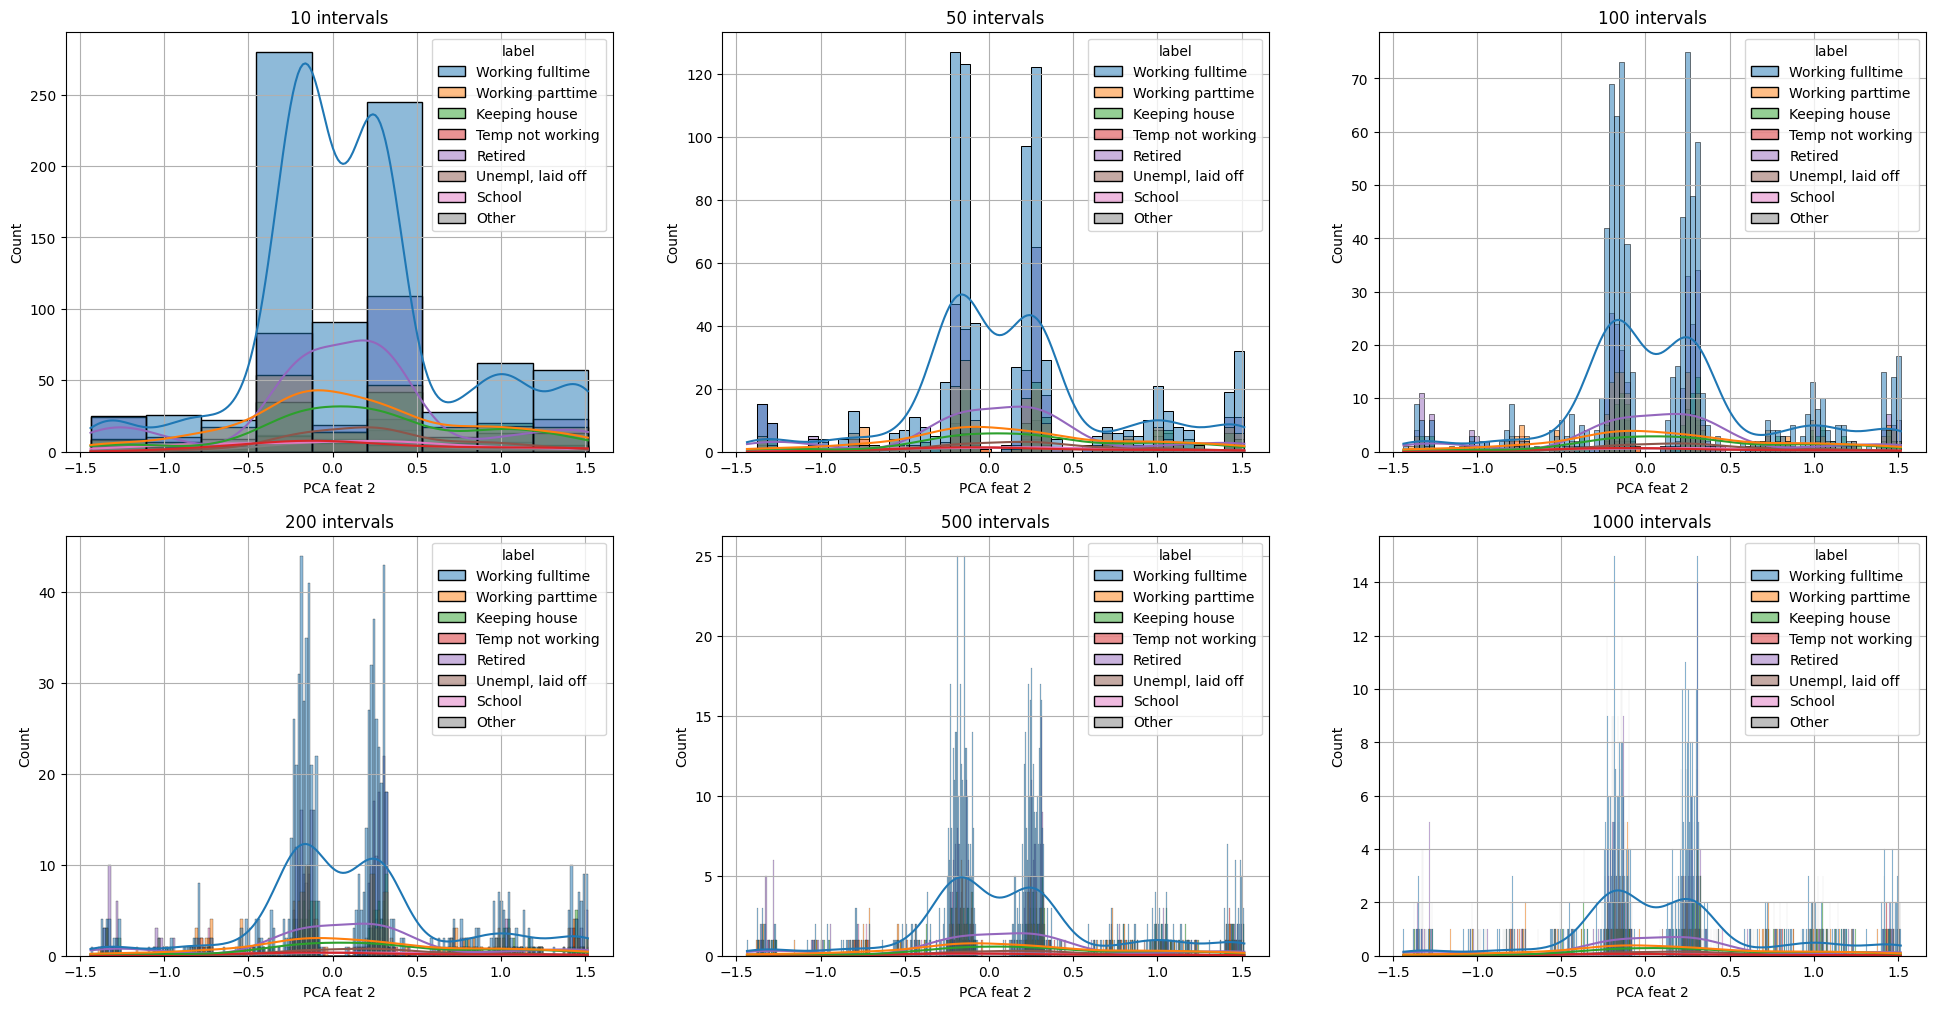
\includegraphics[width=0.75\textwidth]{figures/Thanh/Data_Analysis/Non_null_histogram_PCA_feature_2_vs_wrkstat_labels.png}
    \caption{Histogram của thành phần chính thứ ba tương ứng với từng giá trị dữ liệu trong cột trạng thái làm việc wrkstat}
    \label{fig:Non_null_histogram_PCA_feature_2_vs_wrkstat_labels}
\end{figure}


Hình \ref{fig:Non_null_histogram_PCA_feature_1_vs_wrkstat_labels} và hình \ref{fig:Non_null_histogram_PCA_feature_2_vs_wrkstat_labels} biểu diễn histogram của thành phần chính thứ hai và thứ ba tương ứng với từng giá trị dữ liệu trong cột trạng thái làm việc wrkstat.
Ta thấy hiện tượng tương tự cũng xảy ra với hai thành phần chính thứ hai và thứ ba là phân phối của histogram của các thành phần chính theo các nhóm tương ứng với giá trị trong cột wrkstat gần như cùng hình dạng và trộn lẫn hoàn toàn vào nhau.

Đây là điều rất không mong đợi đối với dữ liệu trong các bài toán phân loại.
Do không thể thấy sự khác biệt về phân phối giữa các nhãn dữ liệu tương ứng, ta rất khó có thể xây dựng một mô hình phân loại tốt.

\begin{figure}[H]
    \centering
    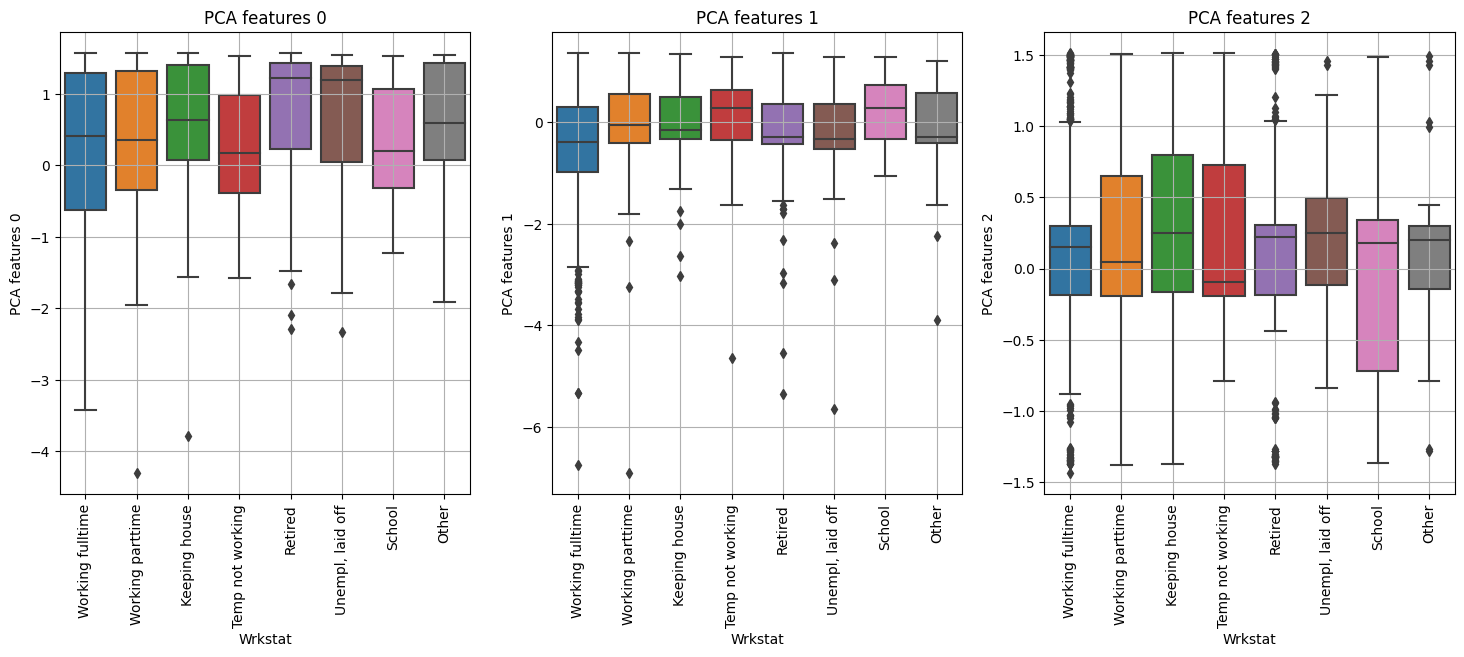
\includegraphics[width=0.8\textwidth]{figures/Thanh/Data_Analysis/Non_null_boxplot_PCA_features_vs_wrkstat_labels.png}
    \caption{Boxplot của các thành phần chính tương ứng với từng giá trị trong cột wrkstat}
    \label{fig:Non_null_boxplot_PCA_features_vs_wrkstat_labels}
\end{figure}

Hình \ref{fig:Non_null_boxplot_PCA_features_vs_wrkstat_labels} thể hiện boxplot của các thành phần chính tương ứng với từng giá trị trong cột wrkstat.
Ta vẫn nhận thấy phân phối của các thành phần chính tương ứng với các nhãn trong cột wrkstat là không có sự tách biệt rõ ràng

\begin{figure}[H]
    \centering
    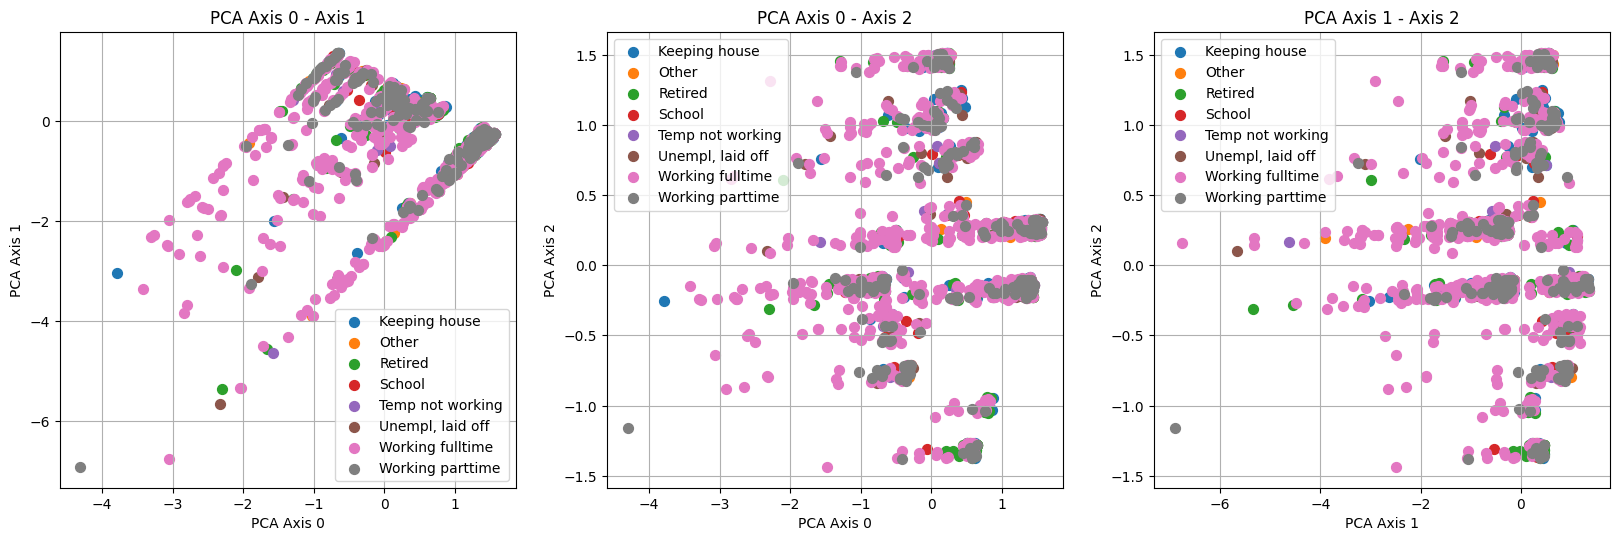
\includegraphics[width=0.8\textwidth]{figures/Thanh/Data_Analysis/Non_null_scatterplot_couples_of_PCA_features_vs_wrkstat_labels.png}
    \caption{Scatter plot của các điểm dữ liệu theo các thành phần chính, màu sắc thể hiện giá trị của cột wrkstat}
    \label{fig:Non_null_scatterplot_couples_of_PCA_features_vs_wrkstat_labels}
\end{figure}

Hình \ref{fig:Non_null_scatterplot_couples_of_PCA_features_vs_wrkstat_labels} biểu diễn scatter plot của các điểm dữ liệu theo các thành phần chính, màu sắc thể hiện giá trị của cột wrkstat.
Ta nhận thấy các quan sát tập trung thành ba, bốn nhóm lớn.
Các nhóm này có dạng dài.
Một điều không may mắn là trong các nhóm lớn thì gần như cũng có sự góp mặt của tất cả các quan sát đến từ các nhãn trong cột wrkstat.

Ta thực hiện phân cụm các quan sát.
Do hình dạng các nhóm có dạng dài, các thuật toán phân cụm theo mật độ sẽ phù hợp.
K-Means không phù hợp trong trường hợp này do K-Means chỉ phù hợp trong trường hợp các cụm có dạng hình cầu.
Ta sử dụng thuật toán DBSCAN.

\begin{figure}[H]
    \centering
    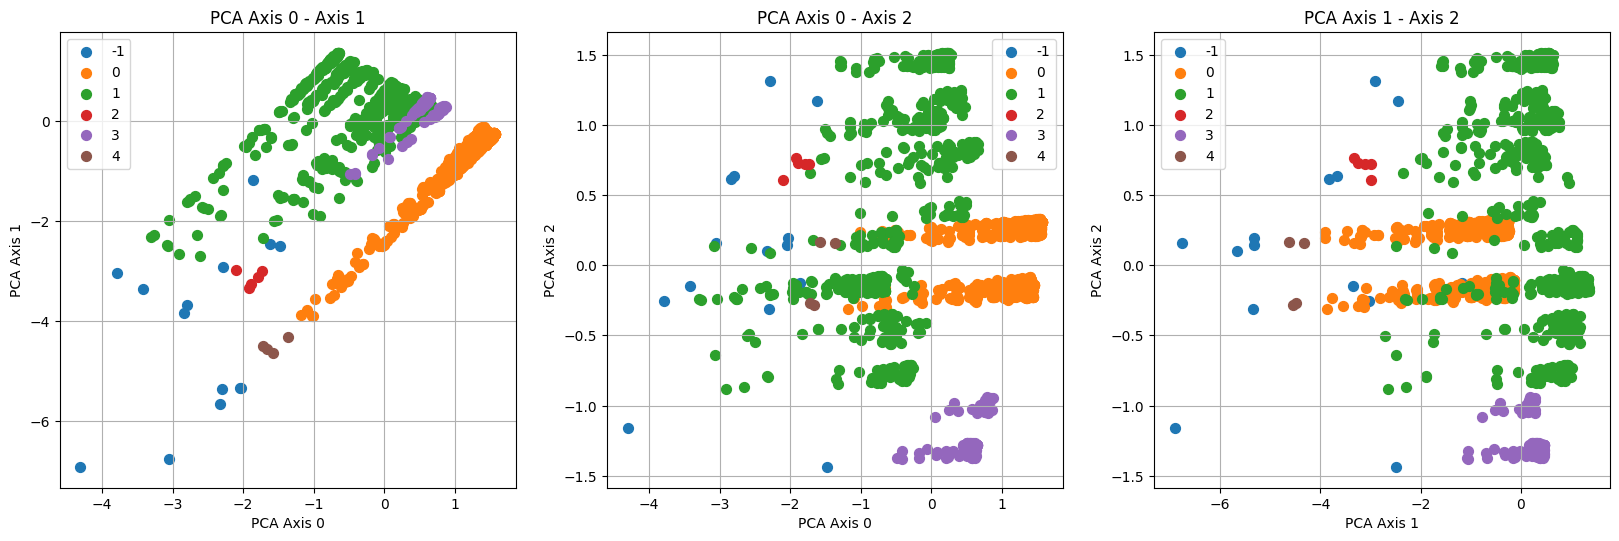
\includegraphics[width=0.8\textwidth]{figures/Thanh/Data_Analysis/Non_null_scatterplot_couples_of_PCA_features_vs_pseudo_clustering_labels.png}
    \caption{Scatter plot của các điểm dữ liệu theo các thành phần chính, màu sắc thể hiện các cụm mà các quan sát được gán vào}
    \label{fig:Non_null_scatterplot_couples_of_PCA_features_vs_pseudo_clustering_labels}
\end{figure}


Hình \ref{fig:Non_null_scatterplot_couples_of_PCA_features_vs_pseudo_clustering_labels} thể hiện Scatter plot của các điểm dữ liệu theo các thành phần chính, màu sắc thể hiện các cụm mà các quan sát được gán vào.
Có ba nhóm chính có số lượng quan sát lớn là nhóm 0, 1.
Ngoài ra còn nhóm 2, 3 và nhóm 4 có số lượng các quan sát ít hơn nhiều 2 nhóm trên.
Nhóm -1 được xem là các điểm ngoại lai.
Ta sẽ xem các nhóm là kết quả của quá trình phân cụm là các nhãn giả và thử một số mô hình phân loại và đánh giá hiệu quả của các mô hình trên tương ứng với các nhãn giả này.

Ta sẽ sử dụng hai loại biểu diễn là các vector ban đầu và các vector được phân tích thành phần chính sử dụng thuật toán PCA từ các vector ban đầu của các quan sát.
Ta sẽ thử ba mô hình phân loại là mô hình Multinomial Logistic Regression, Random Forest và AdaBoost.
Ta chia tập dữ liệu với tỷ lệ 0.6 cho tập train và 0.4 cho tập test.
Ta phân chia theo chiến lược stratify sampling để bảo toàn tỷ lệ của các nhãn trong cả tập train và tập test.


\subsubsection{Multinomial Logistic Regression}

\begin{enumerate}[label=(\alph*)]
    \item Vector thu được từ phân tích thành phần chính sử dụng thuật toán PCA 
    Ta có bảng kết quả huấn luyện mô hình:

    \begin{python}
        precision    recall  f1-score   support

        -1       0.40      0.50      0.44         4
         0       1.00      1.00      1.00       345
         1       1.00      1.00      1.00       272
         2       0.00      0.00      0.00         2
         3       0.97      1.00      0.99        36
         4       0.00      0.00      0.00         1

  accuracy                           0.99       660
 macro avg       0.56      0.58      0.57       660
weighted avg       0.99      0.99      0.99       660

    \end{python}

    và ma trận nhầm lẫn

    \begin{figure}[H]
        \centering
        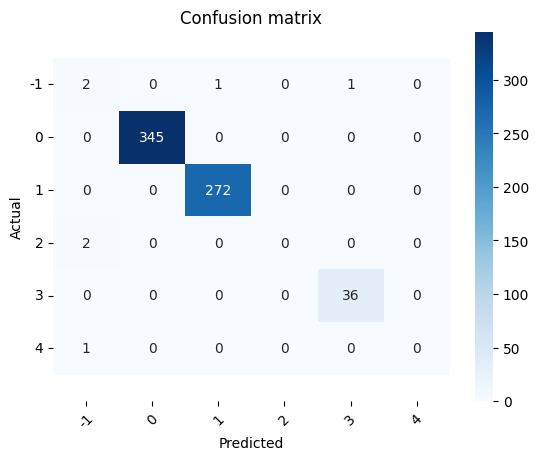
\includegraphics[width=0.6\textwidth]{figures/Thanh/Data_Analysis/Non_null_confusion_matrix_Logistic_PCA_features.png}
        \caption{Ma trận nhầm lẫn của mô hình Multinomial Logistic Regression khi vector đầu vào được phân tích thành phần chính}
        \label{fig:Non_null_confusion_matrix_Logistic_PCA_features}
    \end{figure}

    Ta nhận thấy kết quả phân loại của mô hình vô cùng tốt.
    Các nhóm (cụm) có số quan sát lớn đều có độ chính xác (precision) và độ hồi tưởng (recall) đều bằng 1.

    Ta sẽ phân tích ngược trở lại trọng số của các tham số tương ứng với các đặc trưng của vector ban đầu từ các tham số ứng với các đặc trưng của các thành phần chính bằng công thức:

    \begin{equation*}
        \bold{W} =   \bold{W}_{PCA} \times \bold{U}^T
    \end{equation*}

    với $\bold{W} \in \mathbb{R}^{\mathrm{c} \times d}$, $c$ là số class, $d$ là số chiều của vector ban đầu.
    $\bold{U}$ là ma trận chuyển cơ sở của thuật toán PCA từ không gian $d$ chiều sang không gian $r$ chiều thành phần chính đầu tiên.

    \begin{figure}[H]
        \centering
        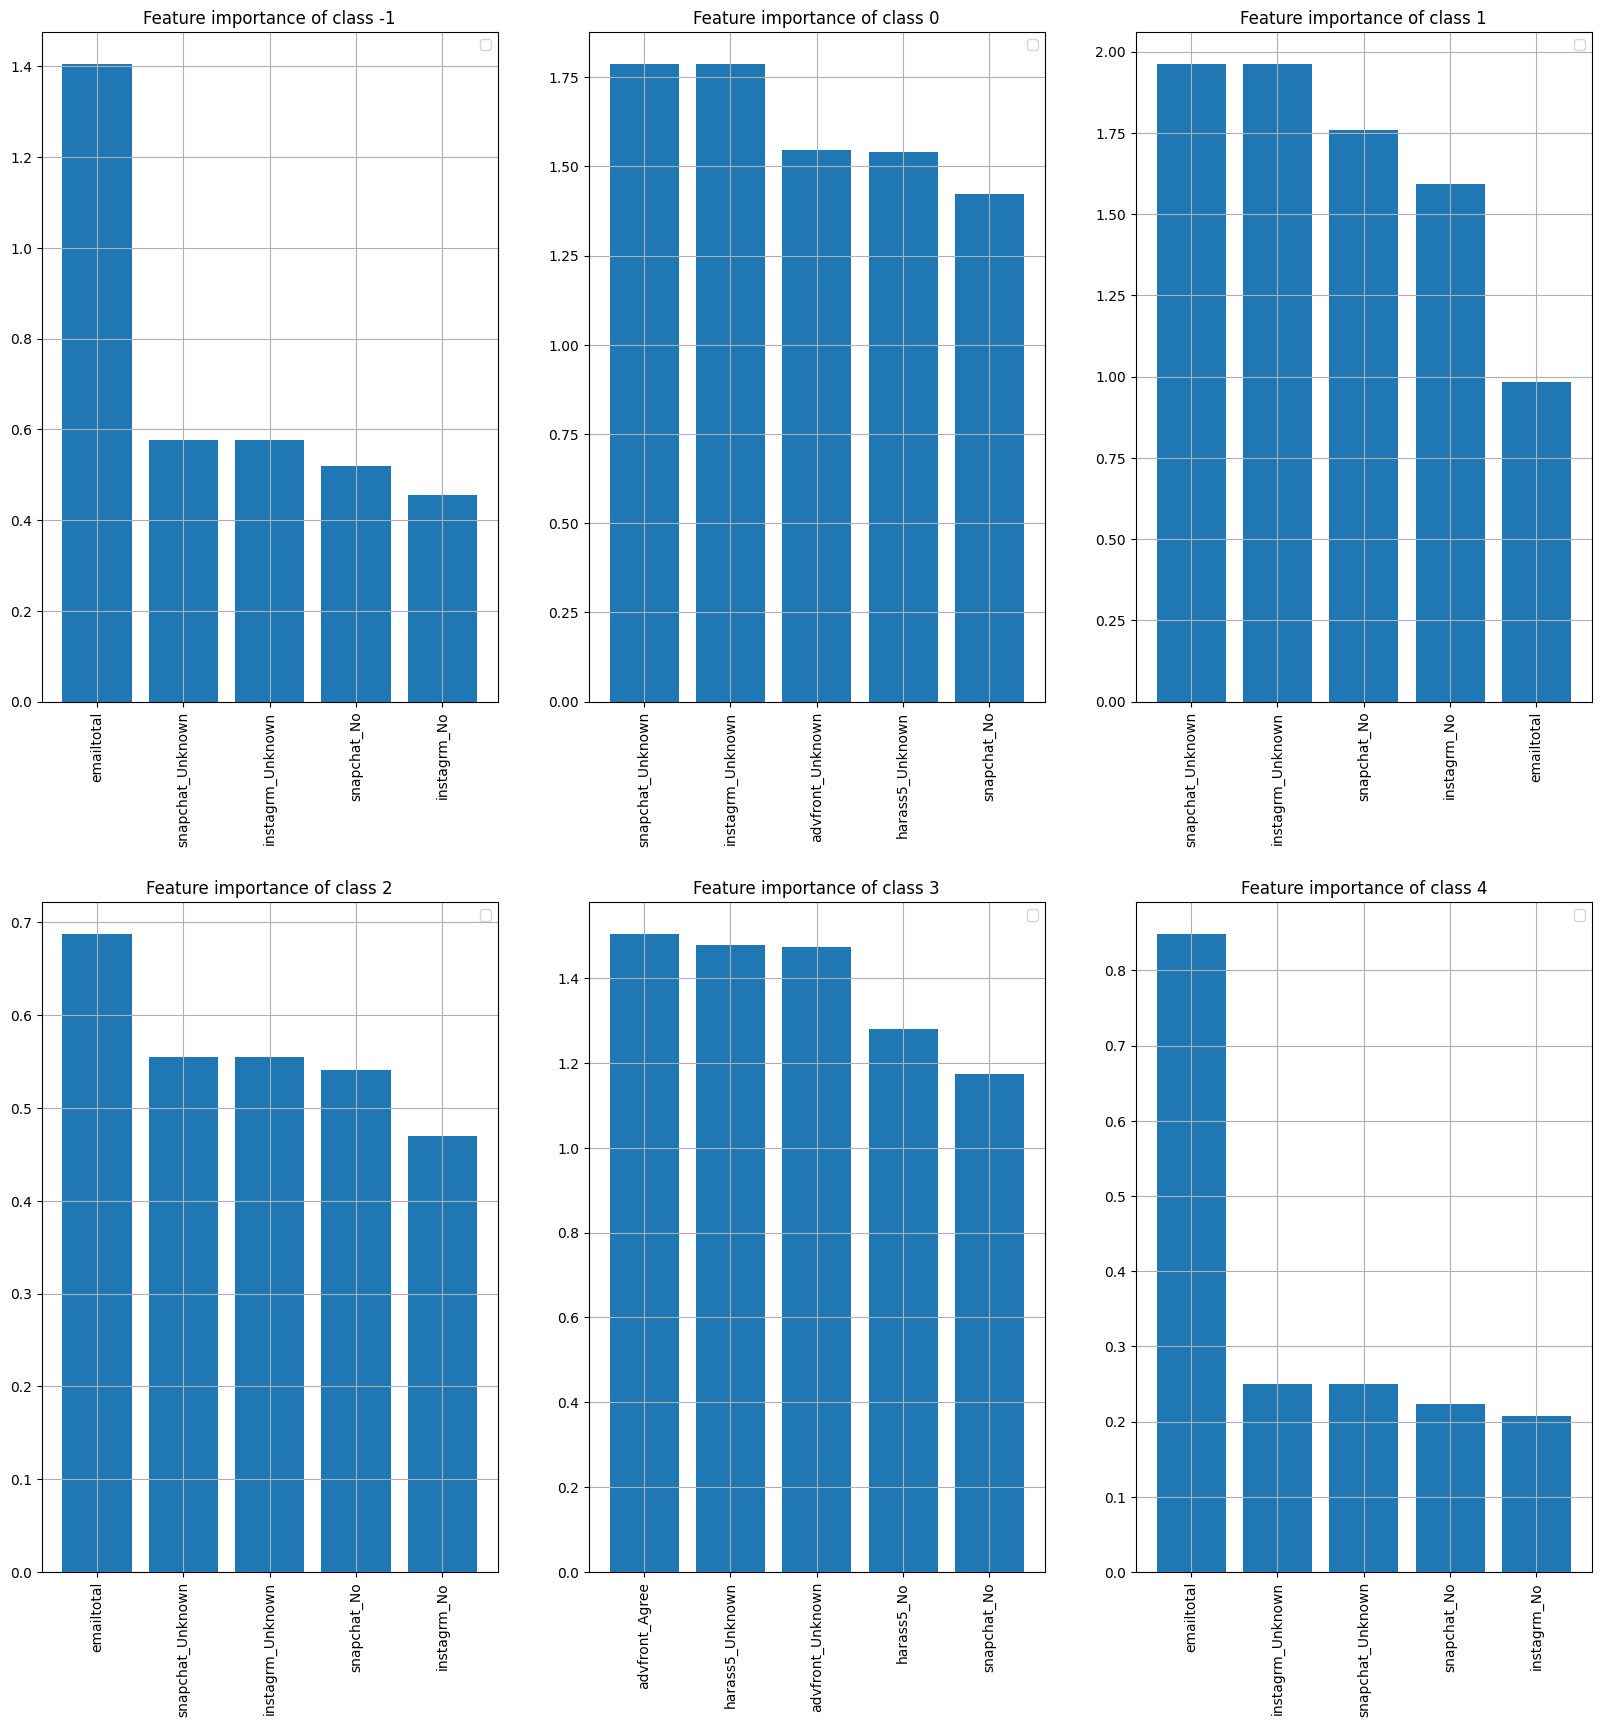
\includegraphics[width=0.6\textwidth]{figures/Thanh/Data_Analysis/Non_null_Feature_Importance_Logistic_PCA_features.png}
        \caption{Biểu đồ cột sắp xếp độ lớn (trị tuyệt đối) tham số của các đặc trưng ứng với từng nhãn giả}
        \label{fig:Non_null_Feature_Importance_Logistic_PCA_features}
    \end{figure}

    Ta có biểu đồ cột sắp xếp độ lớn (trị tuyệt đối) tham số của các đặc trưng ứng với từng nhãn giả thể hiện ở hình \ref{fig:Non_null_Feature_Importance_Logistic_PCA_features}.
    Ta nhận thấy các đặc trưng tương ứng với snapchat\_Unknown hoặc instagrm\_Unknown có trọng số khá lớn.
    Lý do có thể là vì tần suất của các giá trị snapchat\_Unknown và instagrm\_Unknown khá cao (hình \ref{fig:Non_null_frequency_of_unique_values_of_columns})

    \begin{figure}[H]
        \centering
        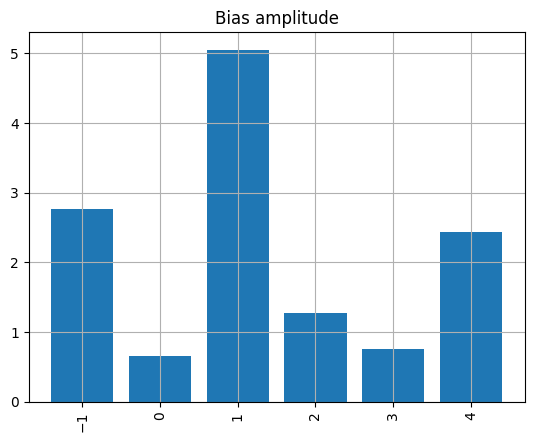
\includegraphics[width=0.6\textwidth]{figures/Thanh/Data_Analysis/Non_null_Bias_Importance_Logistic_PCA_features.png}
        \caption{Biểu đồ cột thể hiện độ lớn của các bias tương ứng với từng nhãn giả}
        \label{fig:Non_null_Bias_Importance_Logistic_PCA_features}
    \end{figure}

    Hình \ref{fig:Non_null_Bias_Importance_Logistic_PCA_features} thể hiện độ lớn của các bias tương ứng với từng nhãn giả,
\end{enumerate}